\renewcommand{\thechapter}{2}

\chapter{Binary Rewriting for Android Apps}

This chapter will introduce Redexer, a binary rewriting tool that
allows static instrumentation of Android binaries. Binary rewriting
enables a wide range of dynamic analyses. Several chapters in this
document utilize Redexer

Rewriting Dalvik bytecode requires significant care. For example, one
common pattern in binary instrumentation is to add sequences of
instructions to methods in key locations (e.g., before method calls or
field lookups). To maintain the original semantics of the method, we
must be careful to ensure that the registers used by the inserted
instructions are not overwriting registers used by the target
method. Redexer provides an API for a programmer to traverse the app's
bytecode and insert instructions without considering these
invariants. It then performs various cleanup passes to ensure the
app's bytecode is corrected.

I begin by describing Redexer in detail. Redexer has been utilized for
both industrial and research applications. After describing Redexer in
detail, I detail one specific use of Redexer, where it is applied to
study location privacy in Android apps. This demonstrates how Redexer
can be applied to provide enhanced security policies on Android apps.

\section{Redexer}
Redexer is a binary transformation framework for Android apps. Android
apps are distributed in the APK file format. Given an input app,
Redexer uses \code{apktool}~\cite{apktool} to unpack the input file
into its constituent files and directories. It then parses each
\code{classes.dex} file into an abstract syntax tree. This allows a
programmer to make changes on a high-level representation of the
bytecode, rather than a compact binary representation. Redexer next
performs a variety of passes to perform bytecode
manipulation. Finally, it dumps out the transformed app and repackages
it as an output APK. In the following subsections, I detail the passes
that Redexer provides to allow app transformation.

\subsection{Parsing Android Bytecode}

As a first stage, Redexer includes a parser for Dalvik
bytecode. Dalvik bytecode files are structured as a series of indexed
``pools'' that contain, among others, strings, types, field
signatures, method signatures, classes, field definitions, and method
definitions. The various pools are tightly intertwined, with many
pointers from one to another, e.g., a method signature contains a list
of pointers to the type pool, and the type pool contains pointers to
elements in the string pool (containing the actual type names).
Dalvik bytecode instructions (which appear in method definitions)
often refer to elements in various pools, e.g., method invocation
instructions include a pointer to a method signature.  Before the
Dalvik Virtual Machine executes a bytecode file, it first
\emph{verifies} it to check that, among other things, the file is
well-formed and the method bodies are type safe.

\subsection{Linking}

Redexer includes an API for statically linking Dex files
together. This allows a programmer to instrument an app by inserting
method calls to a library they write that performs the main work. For
example, Redexer's logging library inserts calls to
\code{Logger.logMethodEntry}, which subsequently performs more complex
work. This makes writing instrumentation simpler by allowing common
utilities to be written in Java rather than bytecode sequences.

\subsection{Modification}
\label{sec:modification}

The modification API allows a programmer to manipulate a Dex file in
various ways. For example, it allows adding and replacing methods,
classes, strings, and other pieces of the Dex file. It also includes
an API to allow inserting bytecode within a method at various
points. 

Inserting code within a method without altering the app's original
semantics is particularly tricky for several reasons. First, whenever
bytecode is inserted into a method at some point, we must be careful
to do so hygenically: the bytecode may not overwrite live variables at
that point. To handle this, Redexer has a utility that allows the
programmer to shift the registers used by a method by some constant
number. This allows the programmer to use the registers within some
range without fear that they are disrupting the state of live
variables at that point.

Unfortunately, register shifting is complicated by the fact that
instructions include bounds on the registers that they can access. For
example, the \code{move} instruction in Dalvik can only address the
first 16 registers. After shifting registers, it is possible that the
method's bytecode will be malformed. One solution might be to add
registers in the upper range of the set of registers used for the
method. However, unfortunately this does not work: the Android calling
convention dictates that the $n$ arguments to the method are put in
the last $n$ registers the method reserves. 

To rectify this problem, Redexer includes a cleanup pass that inserts
the appropriate transformation to move registers into the right
place. For example, a \code{move} instruction will be replaced by a
\code{move-from16} instruction which can address 65k registers. This
is slightly complicated in the case of comparisons, which can only
address the first 16 registers. In this case, Redexer would insert
instructions to move the register from its incorrect position (above
16) into the a register in the lower range. However, this requires
knowing whether or not the register is an object or not,
because---while the comparison bytecode is polymorphic---the move
instructions are not. Using an incorrect move instruction will result
in verification errors. To account for this, Redexer performs dataflow
analysis to recover whether or not the register is an object or not.

Inserting instructions is also tricky because of the way exceptions
are handled within Dalvik. Dalvik exceptions are implemented by
specifying an exception table, which lists ranges of bytecode offsets
to denote try blocks and associates those with exception handlers of a
given type. However, within an exception handler the Dalvik virtual
machine will additionally perform an analysis to ascertain whether it
is possible for each instruction to throw an exception. For example,
Dalvik declares that the \code{move} instruction will not throw an
exception, while an \code{invoke} form might throw an
exception\footnote{the complete listing of bytecode instructions and
  their definitions is given in~\cite{canthrowtable}}.

This presents a subtle complication for bytecode insertion: inserting
\code{invoke} instructions (or other instructions which may throw
exceptions according to the Dalvik VM) may alter control flow, which
subsequently impacts method verification (in particular, extra live
variables may be added which were not present in the original
semantics). To mitigate this, Redexer allows splitting the exception
into two separate handlers: one which ends right before the inserted
instructions, and one which begins after the inserted
instructions.

\subsection{Visitor API and extensions}

The modification API allows manually manipulating the app in various
ways. However, a common rewriting pattern is to traverse the app's
code and perform some operation for each part of the app. To
accomplish this, Redexer includes a visitor API. This allows the
programmer to define some code that will be called for each class
definition, method body, etc... present in the app.

To aid a programmer in constructing instrumentation, Redexer includes
a few utility APIs to recover intra-procedural facts about a method
body. For example, it includes an intra-procedural control-flow
analysis, along with various dataflow analyses and a constant
propagation analysis.

\subsection{Logging}

One particularly useful feature within Redexer is its logging API,
which instruments the bytecode to log an execution of the app. The
logging API is fairly robust and is configurable to log whichever
methods Redexer's user specifies. It is used in several of the
chapters later in this thesis as the basis for app understanding. 

The logging API inserts bytecode before the beginning and at the end
of each method in the app, making a call to \code{logMethodEntry} or
\code{logMethodExit} with the parameters or return value. This allows
recording when specific methods are invoked. API calls are logged in a
similar way: adding a call to \code{logApiEntry} and \code{logApiExit}
before and after the call. 

Note that there are a few complications in inserting these
instructions. First, the instrumented method's code must have its
registers shifted so that the inserted bytecode sequence used to
invoke \code{logMethodEntry} does not overwrite live variables used by
the app. This is done using the modification APIs described in
section~\ref{sec:modification}. We also must perform intra-procedural
control-flow analysis to recover where the end of the method is (if
one exists).

Instrumenting apps with a large amount of logging can be challenging
to do at scale. Apps containing many methods may start to slow down
when logging is not implemented efficiently. There are a few ways to
get around this. For example, logging is configurable via a set of
regular expressions, so the user can choose which subset of methods
are logged. 

In some circumstances, we need to log all methods in a way which
scales to arbitrarily large apps. We found that this can be supported
via using a combination of a worker thread and an efficient buffer to
communicate between them. The logging code is optimized so that it
assembles an array of objects to pass as a data structure to a worker
thread. This is crucial, since the Android OS will kill an app that
suspends the main thread (the thread reacting to app UI requests) if
it becomes too slow. The worker thread then performs the relatively
slow task of serializing the data structure to disk. To communicate
with the code being logged and the worker thread, we use an efficient
lock-free queue (a \code{ConcurrentLinkedQueue} described
in~\cite{Michael:1995}).

\section{An Emperical Study of Location Truncation on Android}
\label{sec:introduction}

This section demonstrates one particular application of Redexer to
study location privacy within Android apps. Many apps use location
information. As implemented today, such apps typically send the device
location over the Internet, and hence users may be understandably
concerned about potential privacy violations. In response, researchers
have developed a number of location privacy-enhancing mechanisms
\cite{Beresford:2004, Shokri:2011, Shokri:2012, Bettini:2005,
  Hoh:2005, Gruteser:2003}, using a range of analytical models to
estimate the degree of privacy and anonymity achieved.

However, there has been much less work \cite{Brush:2010} on
understanding how location privacy-enhancing technology affects the
\emph{utility} of apps---that is, does an app still work well enough
even when location privacy is increased.  I tackle this question by
\emph{directly} measuring how \emph{location truncation}---quantizing
the current location to a user-specified grid spacing---changes the
output of a range of Android apps.

Location truncation is one of the more realistic approaches to
location privacy, with several advantages: It is easy for users to
understand and therefore trust.  It can be implemented easily and
efficiently. And it does not require foreknowledge of the set of
locations to be visited. There are also some disadvantages: Location
truncation primarily defeats localization attacks, rather than
deanonymization or tracking~\cite{Krumm:2009}.  Location truncation
may also be overcome through a combination of prior knowledge (e.g.,
likely movement speeds, locations of road networks, known habits, etc)
and repeated queries over a long period of time~\cite{Gruteser:2005},
\cite{Krumm:2007}.  Even so, we believe that for many everyday uses,
these limitations are not severe for typical users.

While location truncation potentially increases privacy, it may not be
ideal for all apps (e.g., it defeats turn-by-turn navigation), and its
effects may be hard to measure (e.g., for apps that use location to
decide which ads to show).  We retrieved the top \numinvestigatedapps
apps across all categories of the Google Play store, and found that
\numappsusinglocation of these use location. We ran each app to
determine how and why they use location, and found six main
categories: ad localization, listing nearby objects, fine-grained
tasks (e.g., turn-by-turn navigation), geotagging content (such as
pictures), finding the nearest city, and getting local weather
information. (See Section~\ref{sec:usage}.)

Based on this result, we chose to study the effect of location
truncation on apps that produce lists of nearby objects.  These apps
are a good target for a variety of reasons: First, the effect of
truncation is easy to determine, as we can simply look at the output
list. Second, truncation is plausibly useful for these apps: on
Android, most apps do not include internal maps, but rather use
Android's Intent mechanism to ask the Google Maps app to do any
necessary mapping (this was the case for all of the apps in our
study).  Thus, truncating location will help increase privacy of the
user to the subject app, but will not affect the ultimate usage of the
information, assuming that Google and Google Maps are trusted.
Finally, location truncation gives users a very clear tradeoff, in
which they can go a little out of their way in exchange for more
privacy.

We implemented location truncation in \fuzzer{}, a tool built on top
of Redexer. \fuzzer{} modifies a subject app to use a special location
service that snaps reported locations to a latitude/longitude grid
whose spacing is specified by the user. (See Section~\ref{sec:impl}
for details of \fuzzer{}.)

To evaluate how \fuzzer{} affects app utility, we applied it to six
Android apps and measured how their output changed under a range of
conditions.
We developed three different metrics to judge utility of output: The
\emph{edit distance} of the nominal list under truncation compared to
the reference list without truncation; the \emph{additional distance},
which computes how much farther away the first list item in the
nominal list is compared to the reference list; and the \emph{set
  intersection size}, which counts the elements common to the
reference list and nominal list.

We ran each app against \numpointspercity randomly chosen locations
spread across \numcities regions of various sizes, ranging from New
York, NY, population 8.2 million, to Decatur, TX, population
6,000. For each location--region pair, we varied the truncation grid
spacing from 0.1~km to 50~km and measured the result. We found that
the under the additional distance metric, there is typically no change
in app utility up to 1 or 2~km truncation, and that if the user is
willing to go up to 1~km out of their way, most apps can sustain
truncation amounts of 5~km or more. Additionally, the most important
determinant of acceptable truncation was the density of the objects
listed by the app---the lower the density, the more location could be
truncated before seeing an effect.  Across all metrics, most of the
subject apps were able to have their inputs truncated to between 5~km
and 20~km without significantly degrading app utility.

To our knowledge, we are the first to directly and systematically
study how location truncation affects app utility, and our results
suggest location can be truncated to a significant degree without
compromising app utility.

\subsection{How Apps Use Location}
\label{sec:usage}

We began our study by trying to understand how apps use location in
practice. We downloaded the top \numinvestigatedapps most popular free
apps across all categories of the Google Play store as of April 2012,
and found that \numappsusinglocation of these apps request location
permission.  We installed each app on a device or emulator and used
the app, navigating through its screens until we could categorize how
the app uses location information. We identified the following
categories of location usage, summarized in
Figure~\ref{fig:location-uses}:

\begin{itemize}
\item Ads --- Most ad networks deliver location-targeted ads to
  users, and ads are very common on Google Play apps. Thus, this was
  the most popular category of location usage. However, this
  category is not a good subject for our study, as it is
  unclear how to measure the effect of location truncation on ad
  selection. In Figure~\ref{fig:location-uses}, the first row counts
  apps that use location only for ads. Often apps use location both
  for ads and another purpose; the count of these apps is called out
  separately in the remaining rows.
\item Listing nearby objects --- The second most common category of
  location usage is to find some set of objects that are near the
  user's current location. For example, an app might inform the user of
  nearby traffic accidents or construction to avoid. This is the
  category we selected for our study.
\item Fine-grained targeted content --- Many apps require
  very fine-grained location information to provide their service,
  e.g., an app that remembers where the user parked.
  Location truncation is not likely a good idea for these apps.
\item Content tagging or check-in --- Location information is often
  used for geotagging data (e.g., pictures
  or social network posts) or ``checking in'' at the current
  location. For these apps, location truncation is plausible, but
  it is difficult to measure the effect on utility.
\item Nearest city --- Several apps only need to know the current
  location to a very coarse degree, e.g., Living Social and
  Craigslist just need to know the nearest city to select the right
  data to display to the user. Truncating location for these apps
  will have essentially no effect, as they already use coarse data
  (though clearly it might be good from a security perspective).
\item Weather --- Weather apps use the current location to choose
  what weather data to report. We briefly explored the effect of
  truncation on these apps, but found two key problems: First, by
  nature, small
  location changes usually have no effect on weather; and second, weather data changes
  over time, and so it is hard to get consistent data sets because
  our experiments can take a few hours
  to run for each app.
\item Unsure --- There were 17 apps for which we could not determine
  why or how they use location information. These may be cases of
  over-permission, app functionality that we missed in our testing,
  or possibly malicious information gathering.
\item Unable to test --- Finally, we could not test 52 apps because
  they required either telephony-specific features not available on
  our test devices (which did not have phone or data plans) or
  subscriptions to paid services.  For example, many vendors offer
  apps that work only on phones connected to their network.
\end{itemize}

Based on the results of this study, we decided to investigate the
effect of location truncation on apps that list nearby objects, as
this category is common and it is clearly meaningful to measure the
result of truncation on these apps.

\begin{figure}
  \small
  \centering
  \begin{tabular}{|l|rr|}
    \hline
    &
    w/ ads & Total
    \\
%    \hline \hline
%    Top $n$ apps across 24 categories &  & \numinvestigatedapps \\
%    \hline
%    Apps that use location & \numappsads & \numappsusinglocation \\
    \hline \hline
    Only ads & & \numappsonlyads \\
    \hline
    Listing nearby objects & \numappslistads & \numappslist \\
    \hline
    Fine-grained uses & \numappsfinegrainedads & \numappsfinegrained \\
    \hline
    Content tagging & \numappstaggingads & \numappstagging \\
    \hline
    Nearest city & \numappsnearbycitiesads & \numappsnearbycities \\
    \hline
    Weather & \numappsweatherads & \numappsweather \\
    \hline
    Unsure & & \numappsunsure \\
    \hline
    Unable to test & & \numappsnottestable \\
    \hline
  \end{tabular}
  \caption{Location information usage in the top apps}
  \label{fig:location-uses}
\end{figure}

\subsection{Implementation}
\label{sec:impl}

Apps that use location information must request
\code{ACCESS\_COARSE\_LOCATION} or \code{ACCESS\_\-FINE\_\-LOCATION};
the former allows access to a cell-tower--based location and the
latter to a GPS location (if available). \code{FINE\_LOCATION} access
is provided at full device resolution, and \code{COARSE\_LOCATION}
access is truncated to 200 m or 2 km resolution, depending on the
device
parameters.\footnote{\url{https://android.googlesource.com/platform/frameworks/base/+/refs/heads/master/location/java/android/location/Location.java}}
All the apps in our experiments use \code{FINE\_LOCATION}.

We implemented location truncation in the form of \fuzzer{}, a tool
that changes a subject app to receive modified location information.
Location access on Android goes through a fairly narrow API, which
makes it easy for \fuzzer{} to intercept. Apps first request an
instance of class \code{LocationManager}, which includes, among
others, methods to retrieve the last known location and to register a
handler for location updates.  \fuzzer{} controls the granularity of
location information by modifying the subject app so that, instead of
using Android's \code{LocationManager}, it uses a replacement class
provided by \fuzzer{}. This leverages the modification APIs of Redexer
described in section~\ref{sec:modification}. The replacement for
\code{LocationManager} delegates all calls to the system's
\code{LocationManager}, but adds a user-specified amount of truncation
before returning coordinates.

\begin{figure}
  \centering
  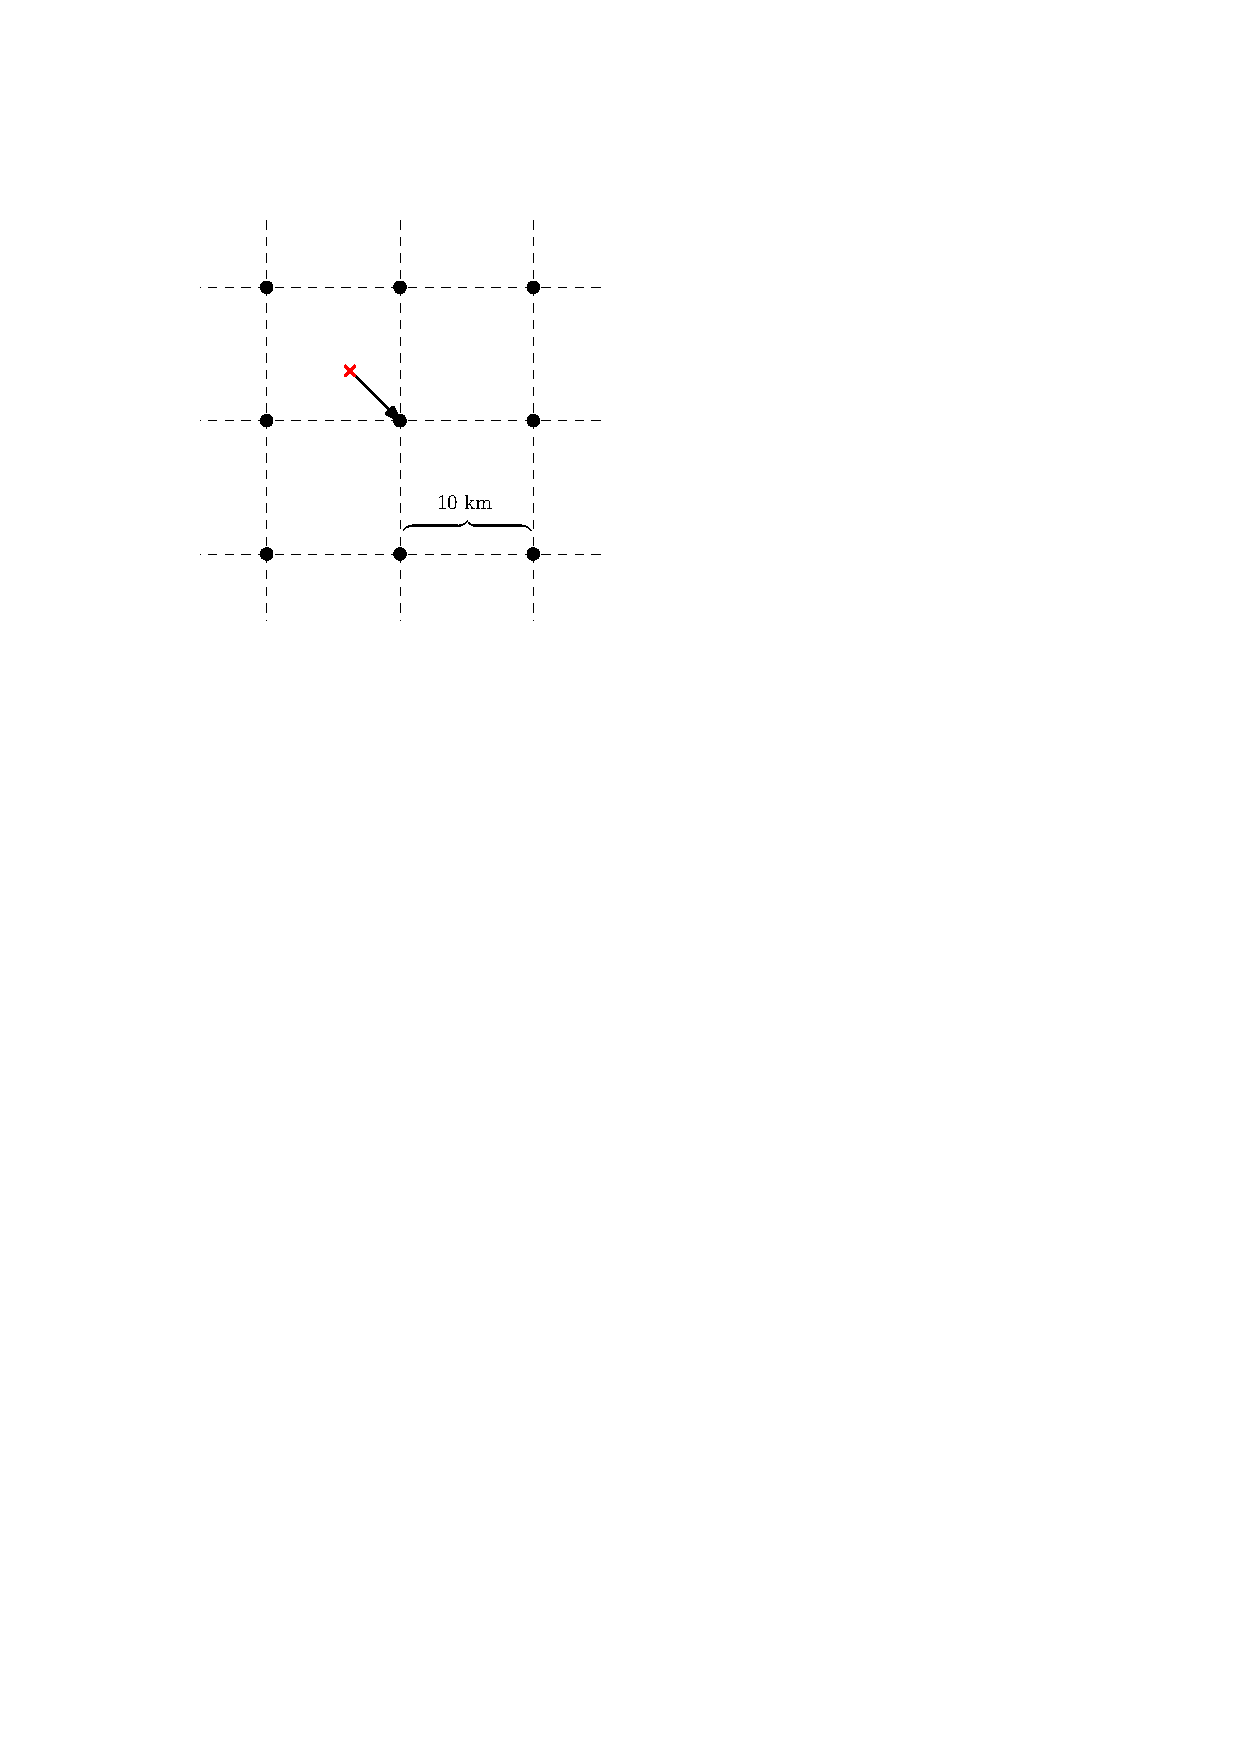
\includegraphics[width=.4\columnwidth]{location_privacy/location_grid_truncation_example}
  \caption{The user (represented by the red cross) has their location
    truncated to a grid of fixed points.}
  \label{fig:grid-truncation-example}
\end{figure}

Once we can intercept calls that pass location information to the app,
it is easy to modify the coordinates however we wish. For our
experiments, we truncate location information, snapping to a
user-specified grid, as illustrated in
Figure~\ref{fig:grid-truncation-example}.  Formally, our
implementation truncates to a grid with spacing $s$ in kilometers
using the formulae:

\begin{displaymath}
  \begin{array}{cc}
%    s_\textit{lat} = s \cdot \Delta^{\textit{lat}} &
    \textit{lat}' = s_\textit{lat} \lceil \textit{lat} /s_\textit{lat} \rceil &
%    s_\textit{long} = s \cdot \Delta^{\textit{long}} &
    \textit{long}' = s_\textit{long} \lceil \textit{long} /s_\textit{long} \rceil
  \end{array}
\end{displaymath}

\noindent where \textit{lat} and \textit{long} are the actual latitude and
longitude, and their primed versions are the new coordinates. Here
$s_\textit{lat}$ and $s_\textit{long}$ are the grid spacing translated
into degrees of latitude and longitude, respectively.
%$\Delta^{loc}$ is number of degrees per meter, which differs for latitude and
%longitude.  
For latitude we use the WGS 84 approximation for North America \cite{latitude-calculator}:

\begin{displaymath}
s_\textit{lat} = \frac{s~\textrm{km}}{111.5~\textrm{km/deg}}
\end{displaymath}

For longitude we use a standard approximation \cite{rapp:geometric}:

\[
s_\textit{long} = s~\textrm{km} \cdot 
  \frac {180 \sqrt{(1 - e^2 \sin^2(\phi))}}
  {\pi a \cos(\phi)}
\]

\noindent where $e^2 = (a^2 - b^2)/b^2$ is the eccentricity of Earth, $\phi$ is
the latitude, $a$ is the radius to the
equator, and $b$ is the radius to the poles.

We verified that \fuzzer{} works correctly in two ways.  First, we 
inserted logging code in \fuzzer{} to give the original position and 
position after location truncation.  We then took the set of locations from our 
testcases, truncated them to varying amounts, and then verified the
resulting positions were correct.  Second, we confirmed that our subject apps'
behaviors changed in sensible ways as we varied the location truncation 
amount.

The Android location manager API also can provide speed information,
which our implementation truncates speed using a similar
formula. However, none of our subject apps use speed
information. Moreover, device-reported speed is often unreliable, so
many apps ignore it, preferring instead to estimate speed using
successive location fixes.

\subsection{Experimental Design}
\label{sec:design}

\begin{figure}
  \small
  %% XXX
  \begin{subfigure}[t]{\columnwidth}
    \centering
    \begin{tabular}{|l|l|}
      \hline
      Name & Objects in List \\ \hline \hline
      \gasbuddy & Gas stations \\
      \restaurantfinder & Restaurants \\
      \hospitals & Hospitals \\
      \webmd & Pharmacies and clinics \\
      \walmart & Stores \\
      \tdbank & ATMs and branches \\
      \hline
    \end{tabular}
    \caption{Descriptions of each subject app.}
    \label{fig:app-descriptions}
  \end{subfigure}

  \bigskip{}

  \begin{subfigure}[t]{\columnwidth}
      \centering
      \begin{tabular}{|l|r|r|}
        \hline
        City & Population & Radius (km) \\ \hline \hline
        New York, NY & 8,200,000 & 30 \\ \hline
        Dallas, TX & 1,200,000 & 20 \\ \hline
        New Haven, CT & 130,000 & 10 \\ \hline
        Baltimore, MD & 620,000 & 12 \\ \hline
        Redmond, WA & 54,000 & 4 \\ \hline
        Decatur, TX & 6,000 & 4 \\ \hline
      \end{tabular}
      \caption{Selected population centers.}
      \label{fig:regions}
    \end{subfigure}

    \bigskip{}

    \begin{subfigure}[t]{\columnwidth}
      \centering
      \begin{tabular}{|r|r|r|r|r|} \hline
        0 km & 0.1 km & 0.2 km & 0.5 km & 1 km \\ \hline
         2 km & 5 km & 10 km & 20 km & 50 km \\ \hline
      \end{tabular}
      \caption{Truncation amounts tested.}
      \label{fig:truncations}
    \end{subfigure}

  \caption{Experimental parameters.}
\end{figure}
 
We conducted a systematic study of the effect of location truncation
on apps that list nearby objects, the largest category in
Figure~\ref{fig:location-uses} for which location truncation's effect is clearly
measurable. We selected a variety of such apps, listed in
Figure~\ref{fig:app-descriptions}, from Google Play. We chose apps
that rely on a variety of different data sets and run under our tool
chain with minimal difficulty.
We then modified each app using \fuzzer, as outlined
in Section~\ref{sec:impl}. Next, we randomly chose a set of locations and
then captured the output list of each app as we varied the current
location and the amount of truncation applied to it. Finally, we used
several metrics to estimate how each truncation affected the app's
utility.

\subsubsection{Locations and truncations}

In a pilot study, in which we examined the results of \fuzzer{} on a
variety of apps, locations, and truncations in an ad hoc manner,
we noticed that truncation has quite different
effects depending on where apps are
run. For example, there is a significantly higher density of restaurants in
a big city than in a rural area, causing one of our subject apps,
Restaurant Finder, to behave very differently under truncation in each locale.
Thus, in selecting locations for
our study, we chose them from a range of population centers of varying
sizes, as shown in Figure~\ref{fig:regions}. 

We modeled each city as a circle centered on the geographical 
city center with a radius estimated
from looking at a map of the region. In
our pilot study, we also found that many apps produce error screens if
given a location that cannot be mapped to a real address, e.g., if the
current location is in the ocean or a heavily forested area.
Thus, we discarded any random points that caused 
problematic outputs from our apps, and randomly picked new
points until we had a set of 10 points that produced correct output
across all apps when the apps were run with no truncation.

For each random location, we ran each app with 10 different truncation
amounts (including no truncation), listed in
Figure~\ref{fig:truncations}.  We chose an upper limit of 50 km because 
many of our subject apps
give results up to or less than 50 km, so the metrics would
be undefined beyond that level.

\subsection{Metrics used for evaluation}
\label{sec:metrics}

Recall from Section~\ref{sec:usage} that we identified apps that list
nearby objects as the best candidate for our study of location
truncation. For example, Figure~\ref{fig:app-example} gives two
screenshots of the Restaurant Finder app being run on a location in
New York, NY (close to Bloomfield, NJ) both without and with
truncation. Here the lists we consider are the restaurants, in order
from closest to farthest, along with their distances.

We explored three ways to measure location truncation's effect on
the output list of such apps: edit distance of the changed list from the
original, the size of the intersection of the original and changed
lists, and the additional distance of the first (closest) list item on
the changed list.

\begin{figure}
  \centering
  \begin{tabular}{cc}
    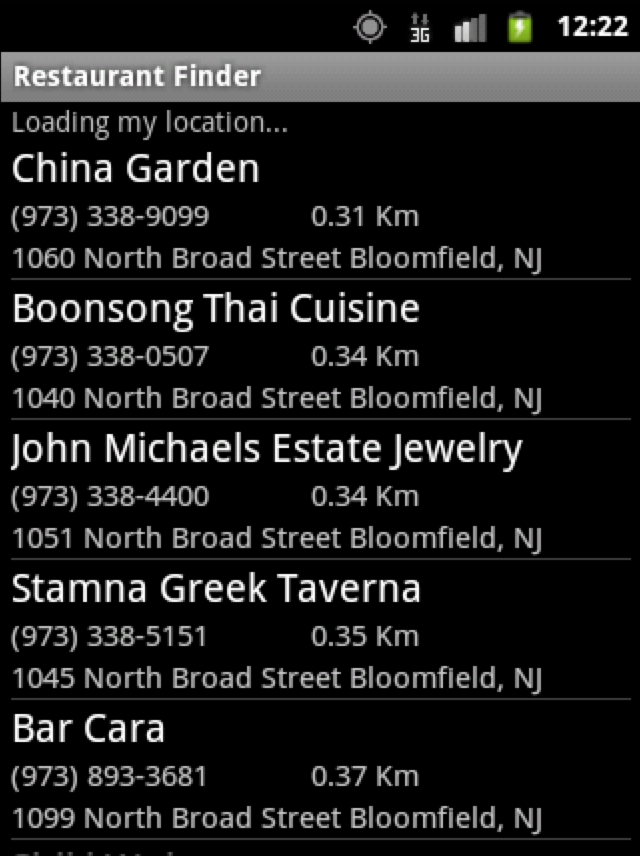
\includegraphics[width=.4\columnwidth]{location_privacy/restaurant_finder_ref_screenshot}
    & 
    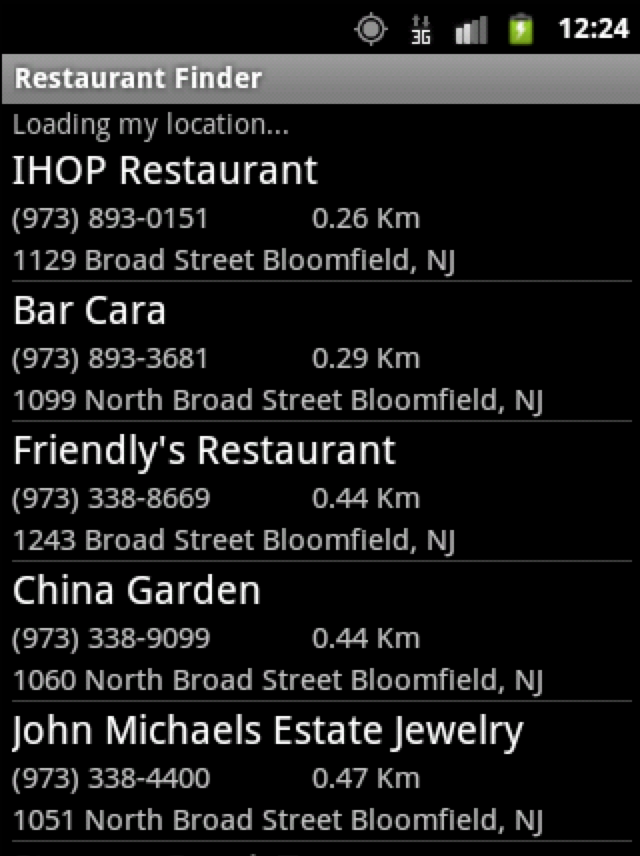
\includegraphics[width=.4\columnwidth]{location_privacy/restaurant_finder_nominal_screenshot}
  \end{tabular}
  \caption{Restaurant Finder without (left) and with (right)
    0.2~km of truncation.}
  \label{fig:app-example}
\end{figure}

\subsubsection{Edit distance}

The first metric we investigated is \emph{edit distance}, which is the
number of edits (insertions, deletions, or swaps) needed to change one
list into another~\cite{levenshtein:1966}. For
example, the edit distance between the lists in
Figure~\ref{fig:app-example} is five, because every item in the
list has changed.

Like the other apps we studied, Restaurant Finder returns more than
one screenful of objects. Thus, in performing our measurements, we
need to decide how much of the app's output to use. We could pick only
the first screen of data, but this restricts edit distance to just
a few possible values. We could pick all the results, but that has the
disadvantage that there could be many changes in the long tail of a
list, yet few users would bother looking that far. Thus, as a
compromise, we opted to compute edit distance over the first four
screens of an app, which we think covers typical usage patterns while
providing useful data.  In each of the apps we tested, this corresponded 
to the first twenty list elements.

\subsubsection{Set intersection size}

Edit distance was the first metric we thought of, but when we tried
measuring it, we found it to be
problematic: Especially on the first screen of data, many locations
are very close, e.g., on the left of
Figure~\ref{fig:app-example}, distances range from 0.31~km to
0.37~km. Yet edit distance would count reorderings of those locations
in the metric.

Thus, we also explored using set intersection size as a metric. We
ignore ordering and compute how many objects are in both the original
and changed list. For example, in Figure~\ref{fig:app-example}, the set
intersection has size three. As with edit distance, we compute the
intersection on the list displayed across the first four screens of
output.

The set intersection metric is also more natural than edit distance in
that it corresponds directly to a common user task of checking whether
some particular object is nearby. For example, we might use Restaurant Finder
to ask, is there any McDonalds nearby, or we might use GasBuddy to
look for the closest Shell station.

\subsubsection{Additional distance incurred}

Ideally, we would like to measure how actual users' behavior is
affected by location truncation, but this is difficult to do without a large
number of human participants. Instead, we developed an \emph{additional
  distance} metric that computes how much farther a user who always
picks the first list item would go given the changed list compared to
the original list.

For example, in Figure~\ref{fig:app-example}, the closest restaurant
is actually China Garden, 0.31 km away. However, under truncation, the
closest restaurant appears to be an IHOP. While the IHOP's reported
distance is 0.26 km, that is the result from the truncated
location---we need to look at the original output list to find out how
far away the restaurant actually is. In this case, IHOP appears on the
second screen of the original list, and it is 0.42~km
away. For this example, then, the additional distance is $0.42 - 0.31
= 0.11$~km.

Restating this more generally, let $D(X)$ be the distance to object
$X$ on the original list. Then the additional distance of a changed
list is $\Delta = D(\textit{First original}) - D(\textit{First changed})$, where
\textit{First original} is the first item of the original list and
\textit{First changed} is the first item of the changed list. Notice
that this metric may be undefined if \emph{First changed} does not
appear on the original list. To reduce the chances of this, we
consider all output screens of an app in computing the metric, and not
just the first four screens. However, in our experiments the metric is
still sometimes undefined for some apps under large truncation amounts.

\subsubsection{Testing infrastructure}

To compute the results of our experiments, we needed to run each
subject app at 60 locations and 10 different truncation
amounts. This is clearly far too many configurations to run by
hand. Instead, we developed testing infrastructure to let us run each
configuration automatically, scrape the resulting output lists, and
then run our metrics on the result.

The core technology we used is Troyd \cite{jsjeon:troyd}, an open
source, black box testing framework that can execute apps (e.g.,
launch them, click buttons, enter text boxes, scroll the screen, etc.)
and gather text from the GUI.  Troyd allows us to write a high level
test case (e.g., to click a sequence of buttons and gather some text)
that can be reused for various test configurations.  We developed a
server that takes an app modified by \fuzzer{}; resigns it with a
shared user ID so that it can be controlled by instrumentation; and
then runs testcases against the app using Troyd.

We ran apps on both Google Nexus S devices and on device emulators;
our infrastructure works the same in both cases, and performing some
runs on actual devices acted as a sanity check. In all cases, the
Android platform was Gingerbread 2.3.3 with the Google APIs, such as
maps, installed. These APIs are special dynamic libraries licensed by
Google and not included on plain Android distributions; these APIs are
needed for the subject programs to run.

We found that, while Troyd mostly did what we wanted, we needed to
extend it to handle additional GUI elements.
For example, while Troyd can capture the currently visible GUI elements,
many \code{Views} (such as those in \code{ListView} elements) are 
reused, and their contents only appear when the screen is scrolled.
Thus, we extended Troyd with special functionality to 
navigate to screens that may have unrendered information.
We also found that, as is usual in large-scale
testing, 
experimental tests sometimes failed unpredictably, e.g., an emulator
or device would crash for no apparent reason. These are likely due to
subtle bugs lurking in the OS or emulator implementation that
were tickled by the experiment's atypical usage pattern. Thus, our
testing infrastructure catches any failed runs and reschedules those
experiments to be run again. Finally, our testing infrastructure allows
multiple experiments to be done in parallel; the majority of the
experiments were done on a machine with six Intel Xeon processors, 
each with four cores, and 48 GB of RAM.  Each individual test took on
the order of a few minutes to run, depending on the app.
Our tests ran up to fifteen emulators at once.

\begin{figure*}[t!]
  \centering
  \begin{tabular}{ccc}
    
    \begin{minipage}{2in}
      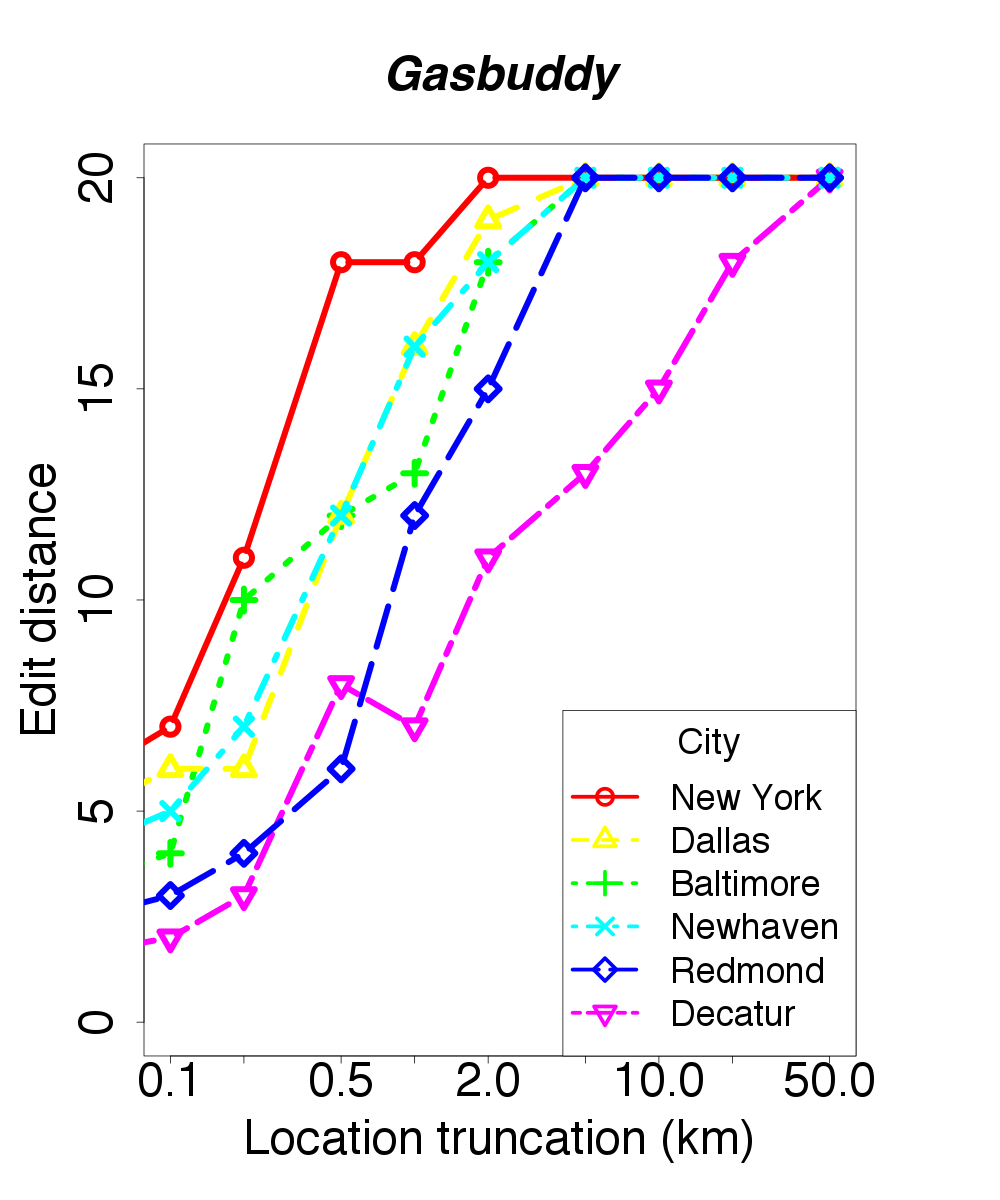
\includegraphics[width=\textwidth]
                      {location_privacy/data/gasbuddy/plots/medians_across_city_20}
    \end{minipage}
    
    % [width=.6\textwidth]
    \begin{minipage}{2in}
      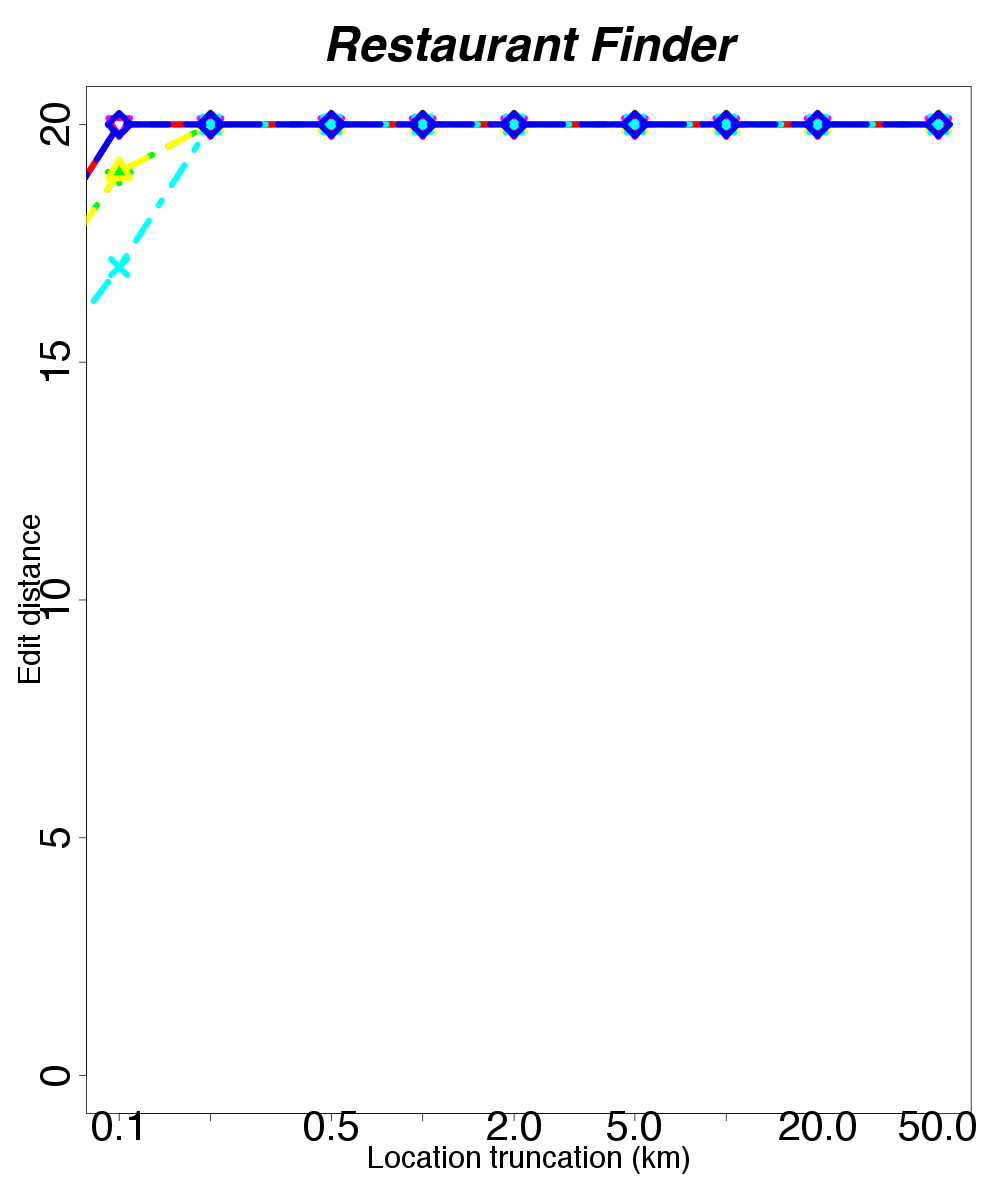
\includegraphics[width=\textwidth]
                      {location_privacy/data/restaurant_finder/plots/medians_across_city_20}
    \end{minipage}
    
    \begin{minipage}{2in}
      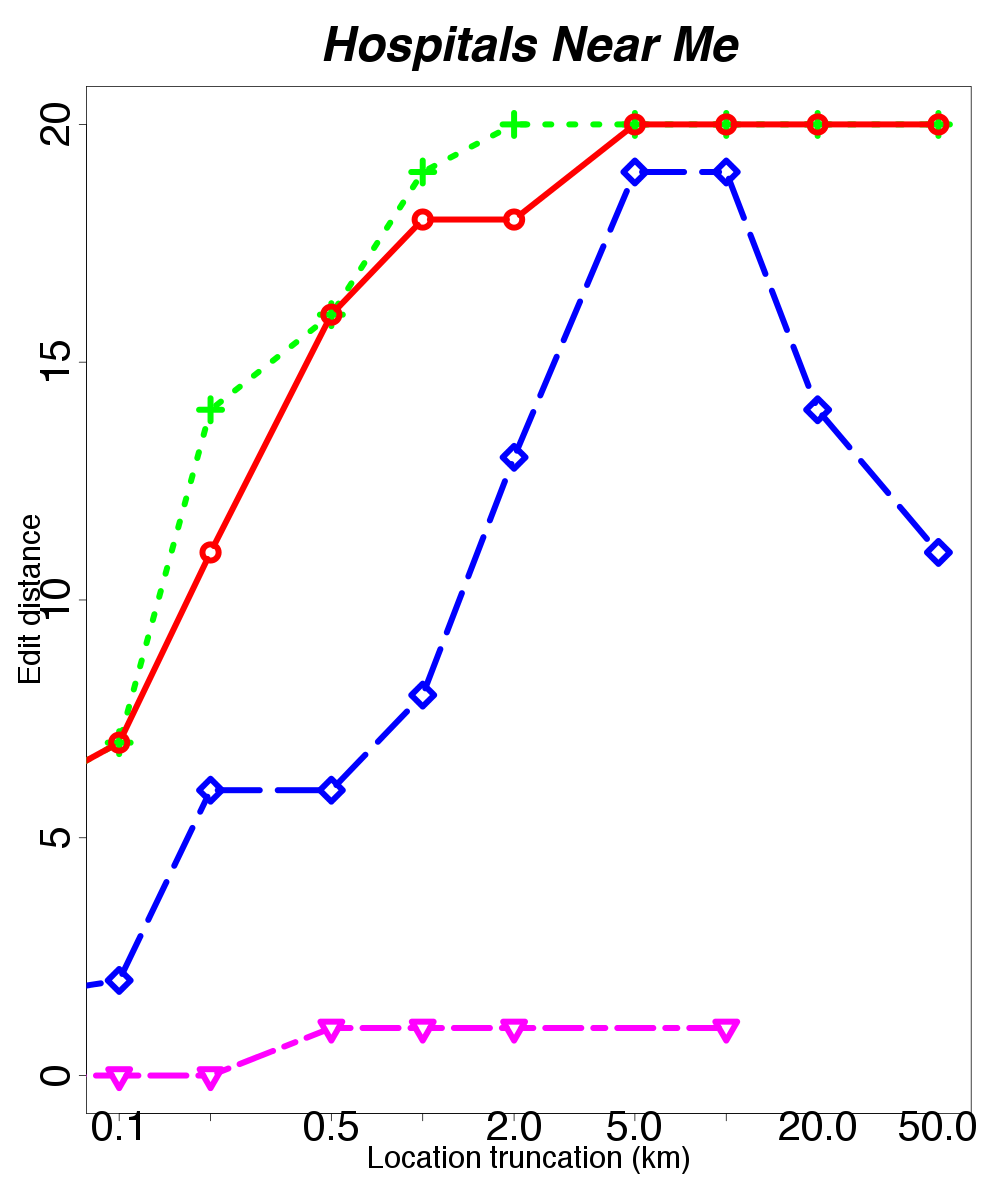
\includegraphics[width=\textwidth]
                      {location_privacy/data/hospitals/plots/medians_across_city_20}
    \end{minipage}
    
    \\
    \begin{minipage}{2in}
      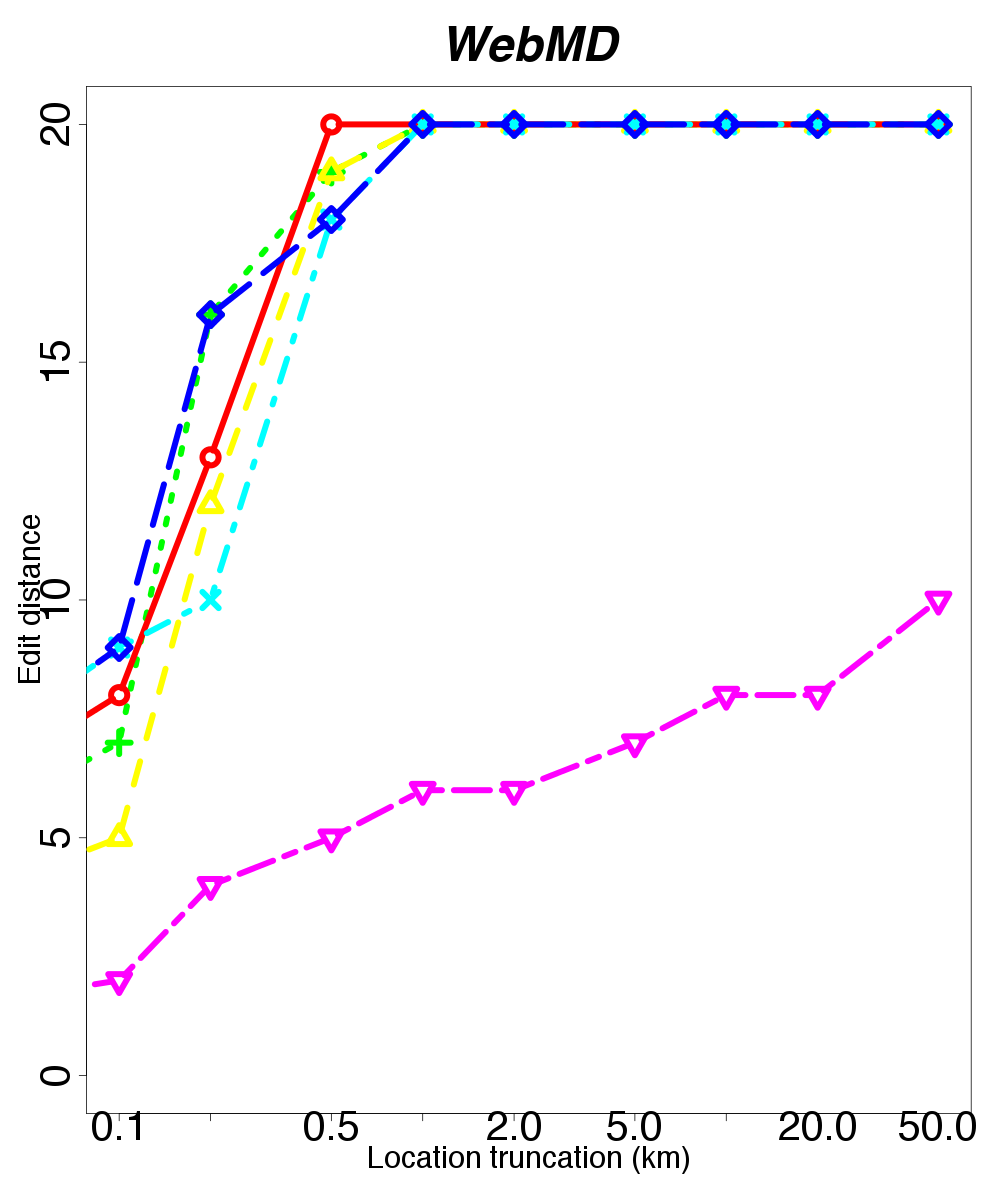
\includegraphics[width=\textwidth]
                      {location_privacy/data/webmd/plots/medians_across_city_20}
    \end{minipage}
    
    \begin{minipage}{2in}
      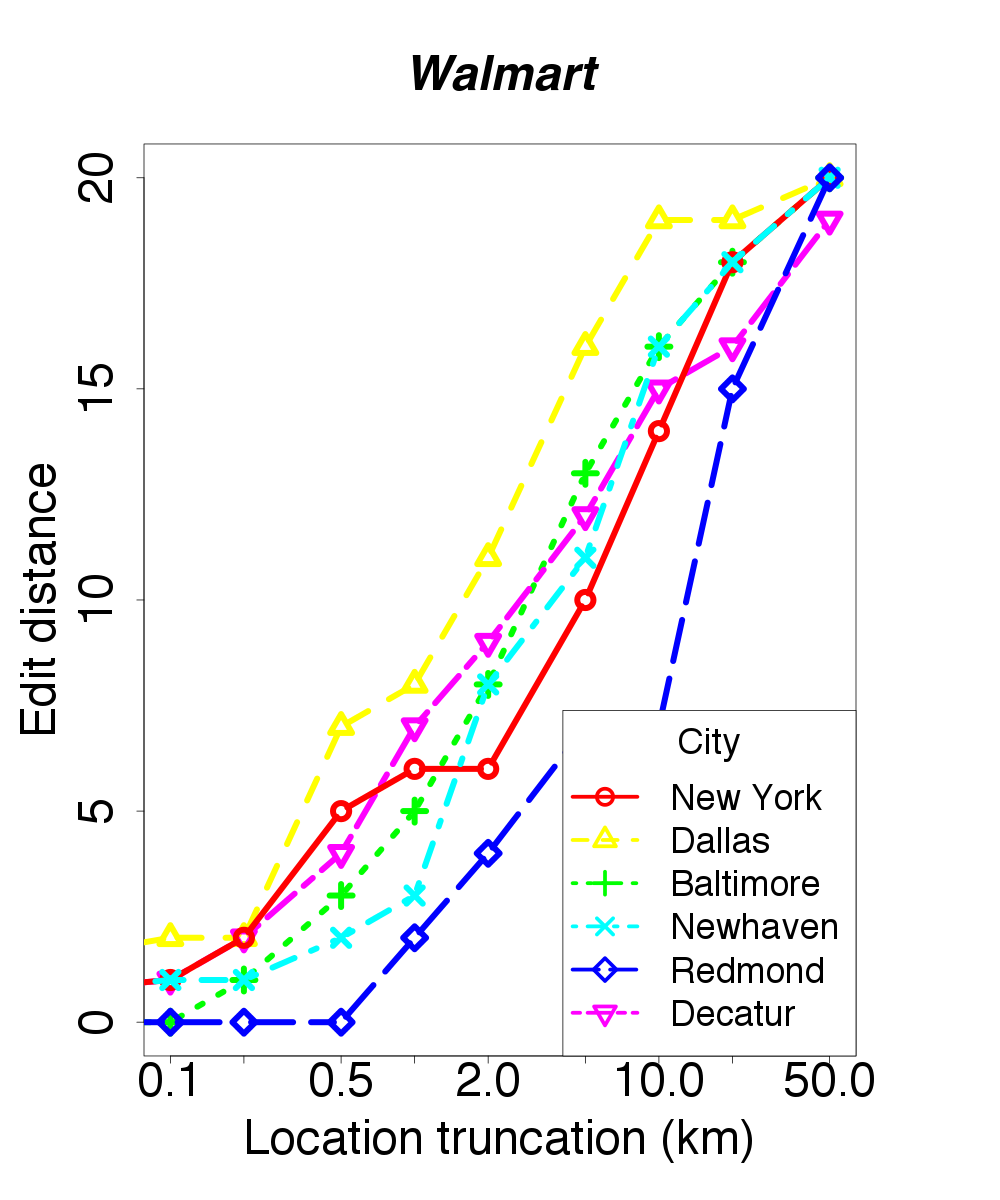
\includegraphics[width=\textwidth]
                      {location_privacy/data/walmart/plots/medians_across_city_20}
    \end{minipage}
    
    \begin{minipage}{2in}
      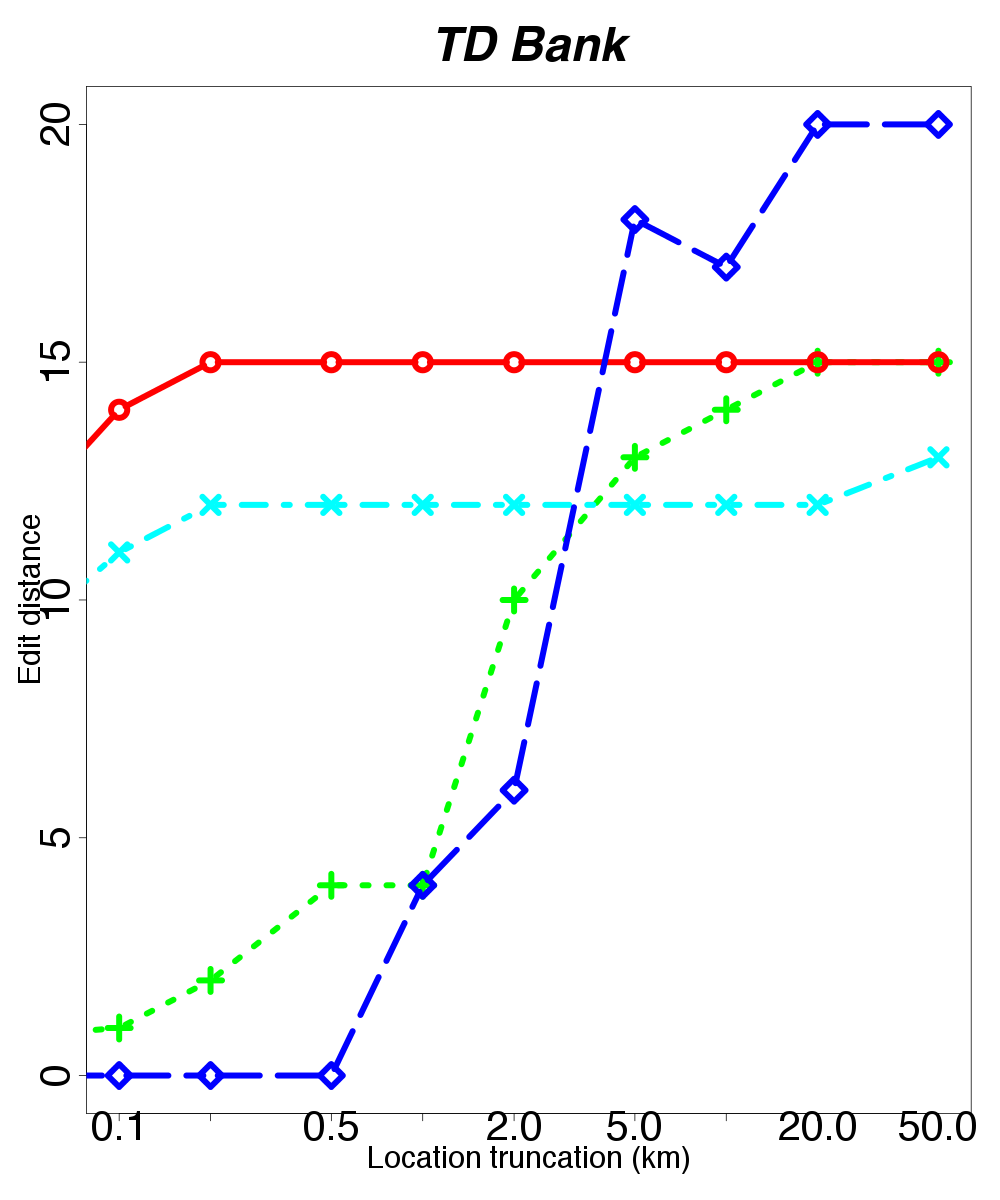
\includegraphics[width=\textwidth]
                      {location_privacy/data/tdbank/plots/medians_across_city_20}
    \end{minipage}
  \end{tabular}
  \caption{Graphs of median edit distance versus truncation
    amount. Higher edit distance implies lower utility.}
  \label{fig:edit-distance-metric}
\end{figure*}

\subsection{Results}
\label{sec:results}

Finally, we present the results of our study. At a high level, we
found that across our
subject apps and locations, location can be
significantly truncated without significantly harming utility: up to 20~km
when an app is used in a lower population area, and usually (for five of six apps) 
at least 5~km in more populous areas.  We also found that apps have relatively little 
change in utility up to a certain amount of truncation, typically
about 5~km, after 
which the app's output becomes much less usable.  Finally, we found that the factor 
that most determines the ability to truncate location was the density
of the set of locations the app computes over.

In the discussion that follows, we include several plots. In each
plot, the $x$-axis is the truncation amount; note that because of our
choice of truncations, this axis is essentially log-scale.  The $y$-axis
is the median of one of our metrics on the 10 randomly chosen points
for each population center.

We next consider each of our three metrics in turn.

\begin{figure*}[t!]
  \centering

  \begin{subfigure}[t]{\textwidth} 
    \begin{tabular}{ccc}
    
    \begin{minipage}{2in}
      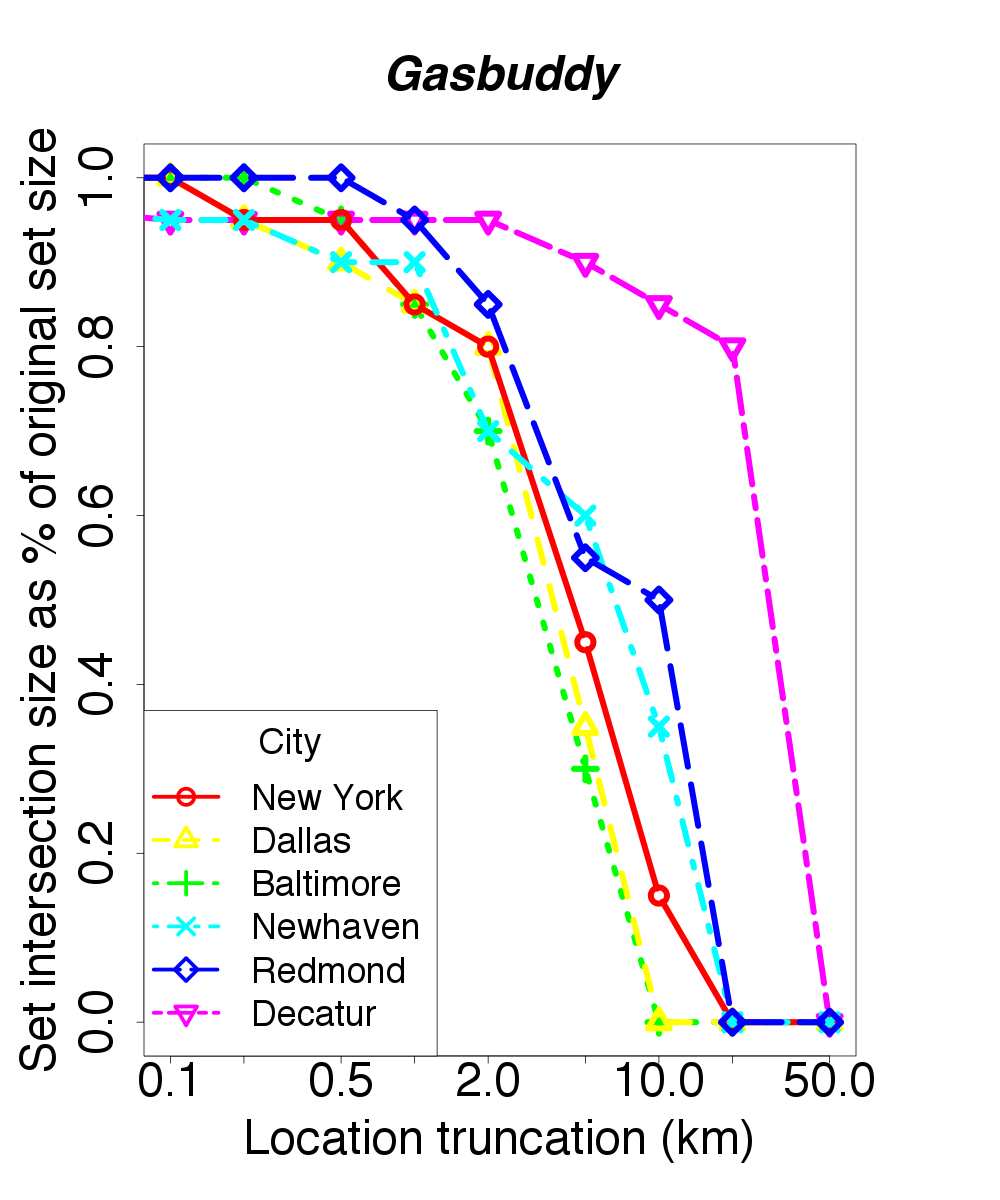
\includegraphics[width=\textwidth]
                      {location_privacy/data/gasbuddy/plots/medians_across_city_si_20}
    \end{minipage}
    
    % [width=.6\textwidth]
    \begin{minipage}{2in}
      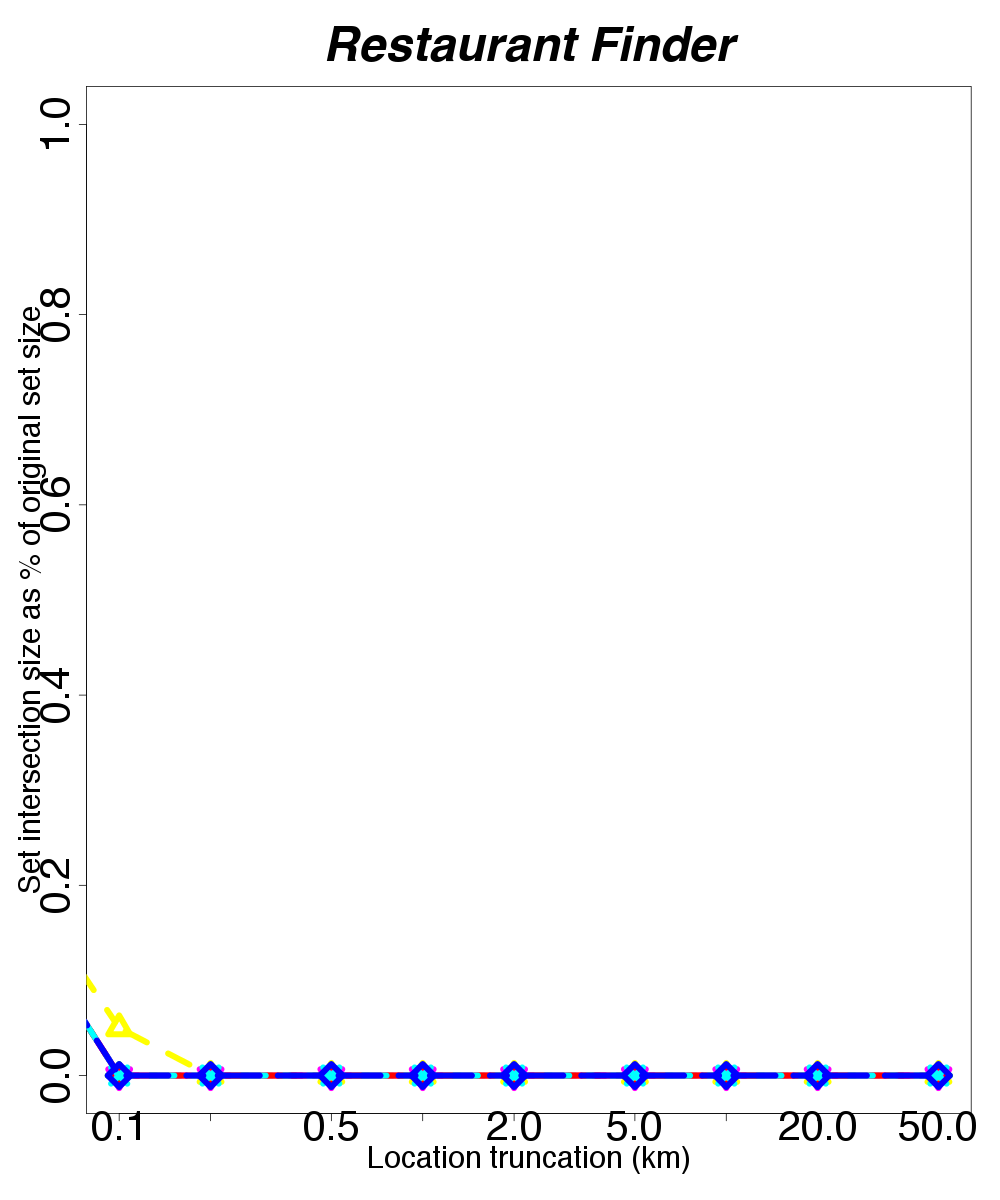
\includegraphics[width=\textwidth]
                      {location_privacy/data/restaurant_finder/plots/medians_across_city_si_20}
    \end{minipage}
    
    \begin{minipage}{2in}
      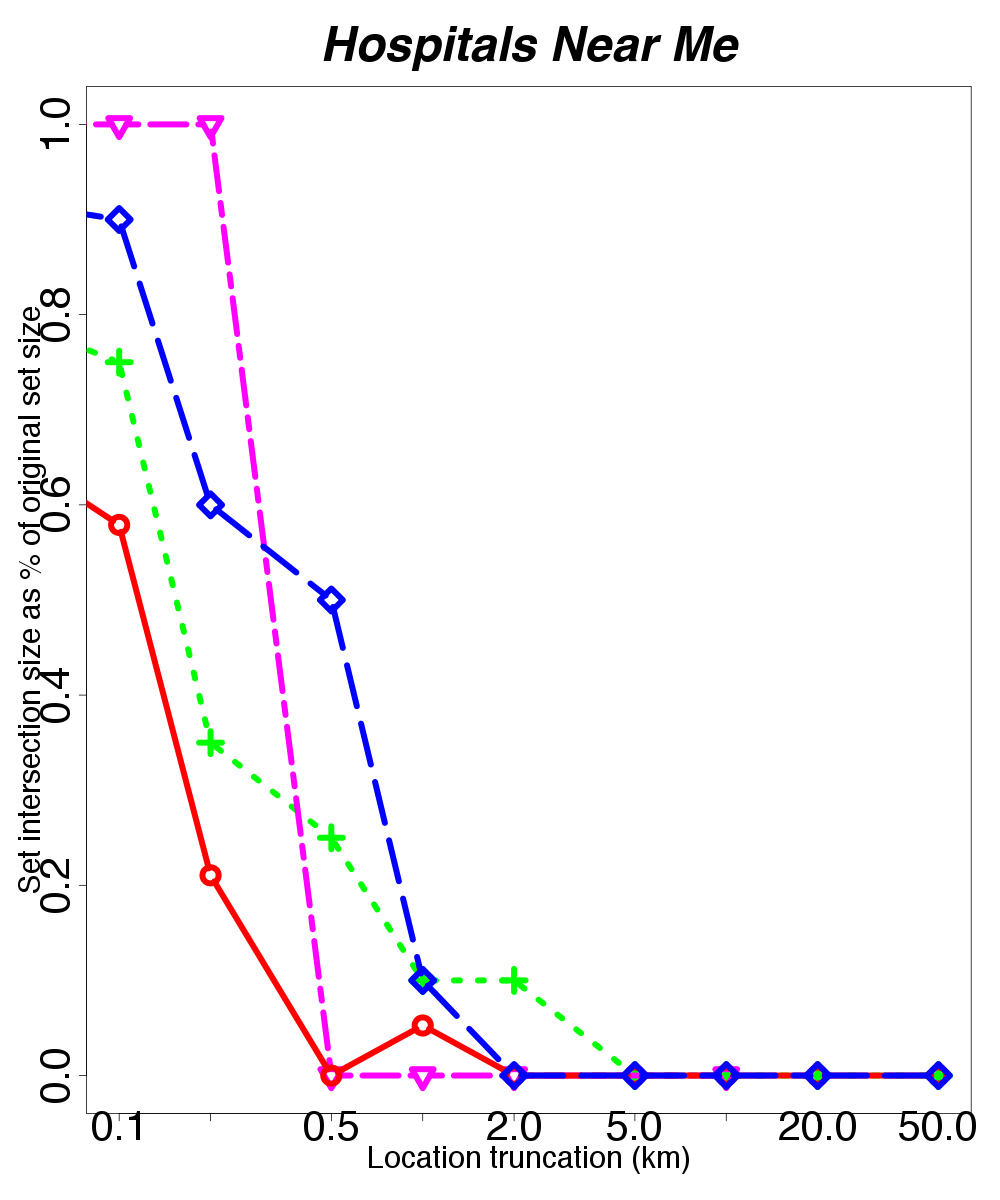
\includegraphics[width=\textwidth]
                      {location_privacy/data/hospitals/plots/medians_across_city_si_20}
    \end{minipage}
    
    \\
    \begin{minipage}{2in}
      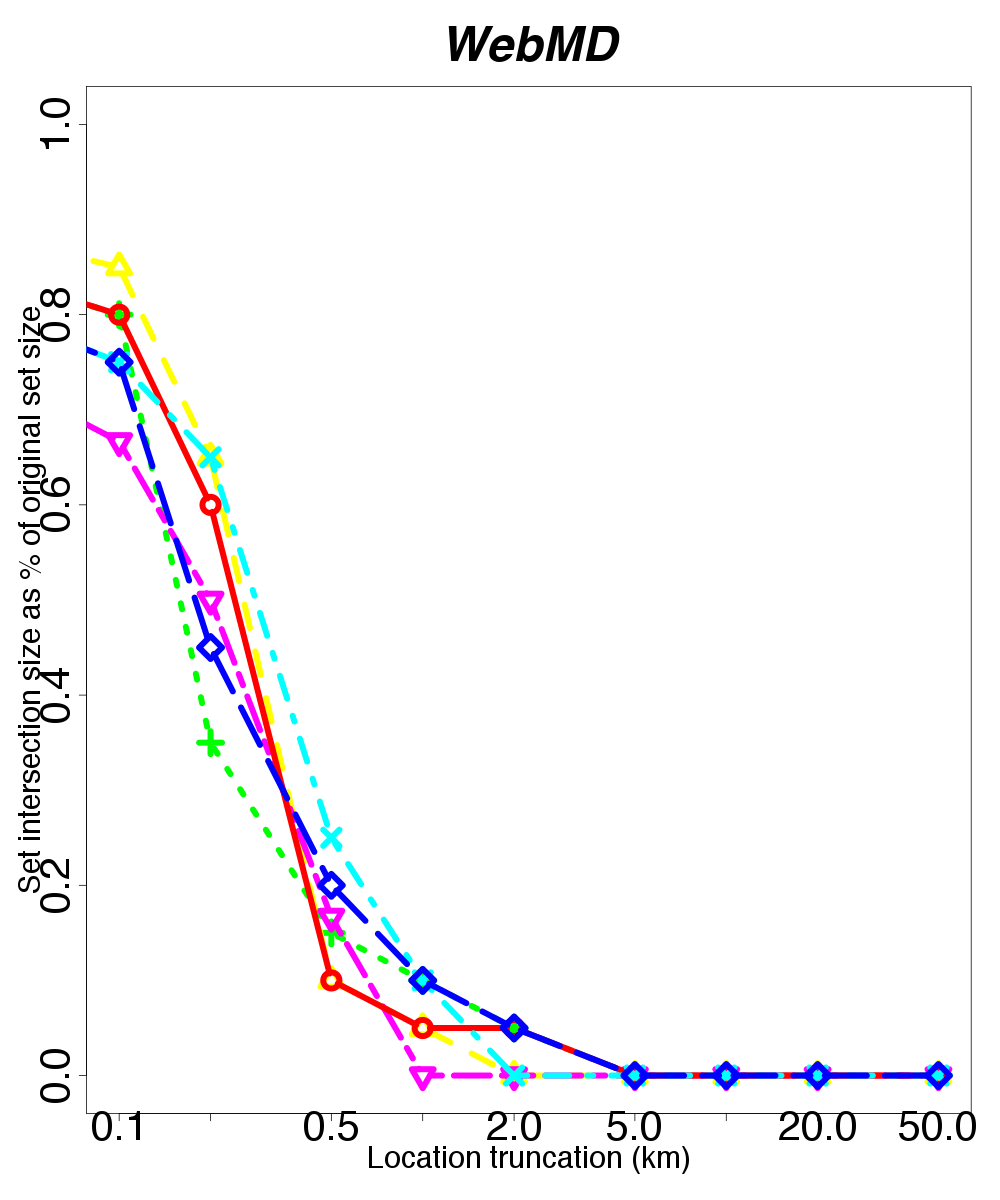
\includegraphics[width=\textwidth]
                      {location_privacy/data/webmd/plots/medians_across_city_si_20}
    \end{minipage}
    
    \begin{minipage}{2in}
      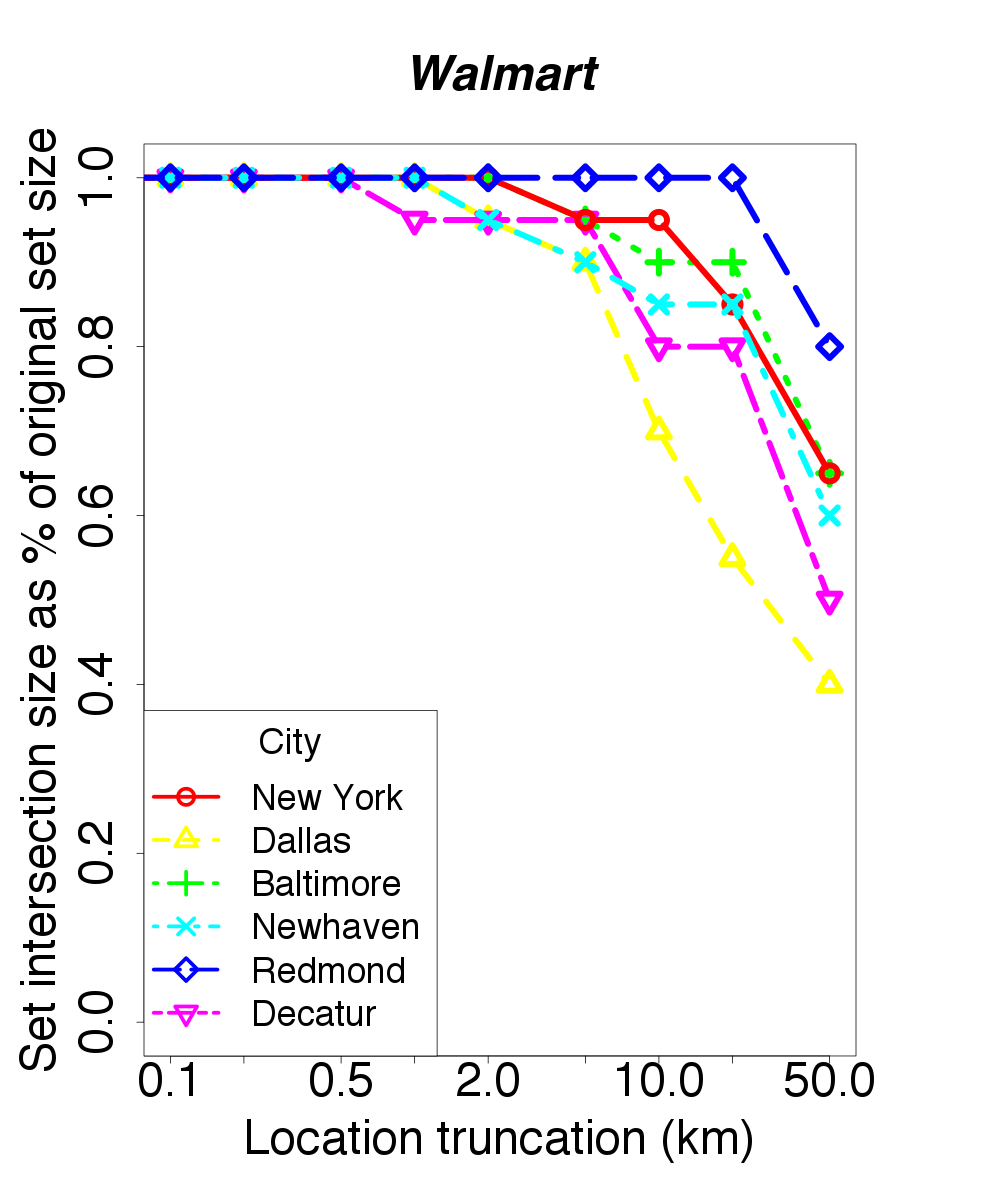
\includegraphics[width=\textwidth]
                      {location_privacy/data/walmart/plots/medians_across_city_si_20}
    \end{minipage}
    
    \begin{minipage}{2in}
      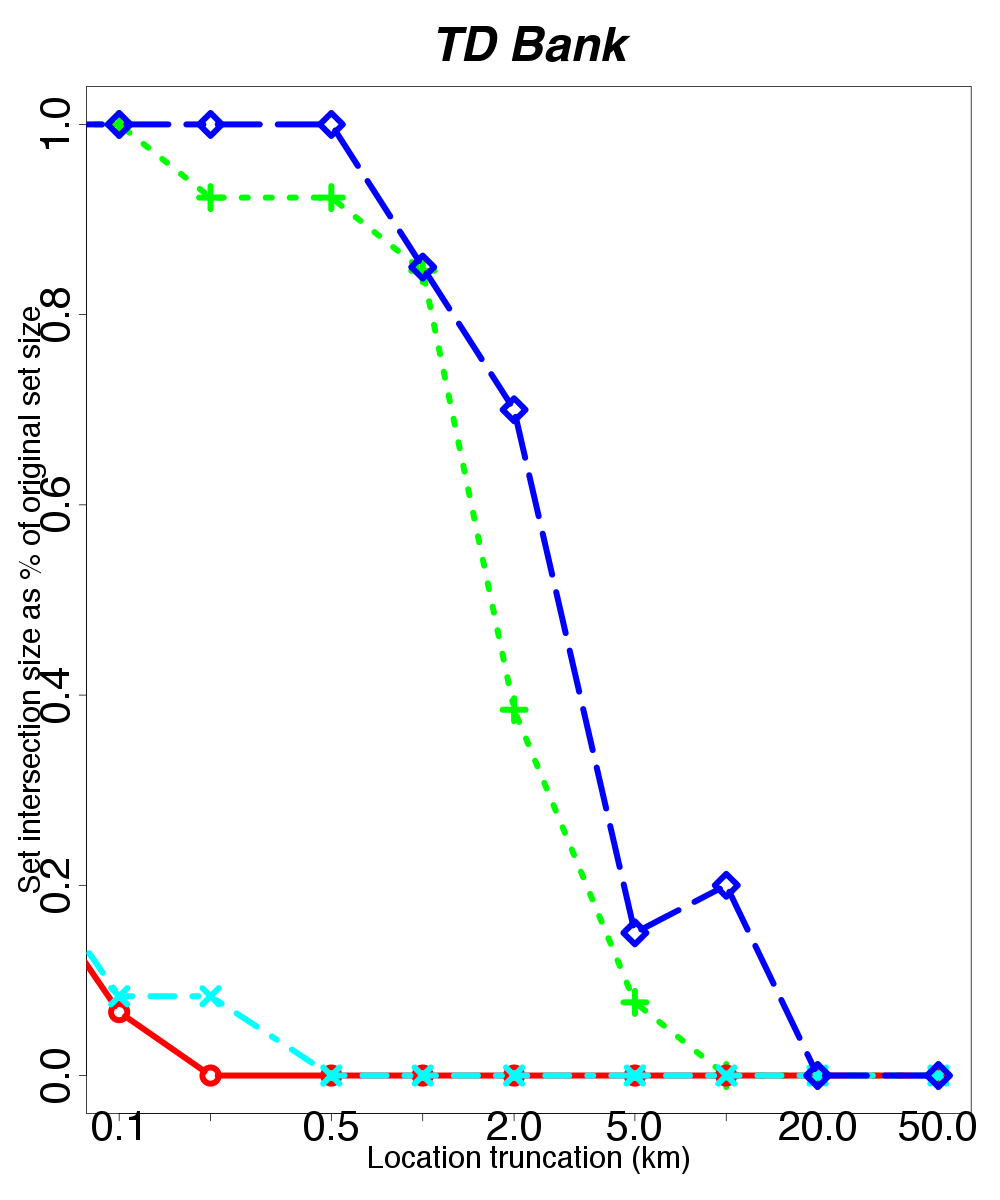
\includegraphics[width=\textwidth]
                      {location_privacy/data/tdbank/plots/medians_across_city_si_20}
    \end{minipage}
  \end{tabular}
  \caption{Graphs of median set intersection size versus
    truncation amount. Lower set intersection size indicates lower
    utility.}
  \label{fig:set-intersection-metric}
  \end{subfigure}

  \bigskip{}

  \begin{subfigure}[t]{\textwidth}
 \small
 \centering
 \begin{tabular}{|l|rrrrrr|}
 \hline
 & New York & Dallas & Baltimore & New Haven & Redmond & Decatur \\
 \hline
 Gasbuddy & 5 & 5 & 2 & 2 & 5 & 50 \\
Restaurant Finder & 1 & 0.5 & 0.1 & 0.1 & 0.1 & 0.2 \\
Walmart & 50 & 10 & 50 & 50 & $\cdot$ & 50 \\
TD Bank & 10 & $\cdot$ & 50 & 20 & $\cdot$ & $\cdot$ \\
WebMD & 10 & 5 & 2 & 10 & 10 & 50 \\
Hospitals Near Me & 5 & $\cdot$ & 20 & $\cdot$ & 20 & $\cdot$ \\
\hline

\end{tabular}
 \caption{Largest truncation amount (km) before which the median set
   intersection size is lower than 80\%.}
 \label{fig:knee-points-set-cutoff}
  \end{subfigure}
  
  \caption{Set intersection size results.}
\end{figure*}

\subsubsection{Edit Distance}

Figure~\ref{fig:edit-distance-metric} shows how edit distance 
 varies
on our location set.  
Note that Hospitals Near Me and TD Bank do
not have data for cities for which the app did not generate enough output
to calculate a significant result. 
For example, there are no TD banks in Dallas.  In some cases,
TD Bank and Hospitals Near Me do generate data, but they generate 
a very small set of results (Hospitals Near Me only returns hospitals
within 50 miles, for example).
Thus, edit distance appears to go down
at large truncation values because in less populous 
locations they output smaller sets of locations.

The plots show that in most cases, the output lists change to some
degree even at the smallest truncation level. Moreover, in two cases
(Gasbuddy and Restaurant Finder), the edit distance quickly reaches
its maximum value (all items in the list change) in several
locales. WebMD is similar, though it plateaus somehwat later. The
remaining three apps, in contrast, show a generally steady progression
of edit distance versus truncation amount.

The reason for these trends is density of objects--Gasbuddy,
Restaurant Finder, and WebMD all return lists of items that can
commonly be found everywhere, whereas there may be only a few
hospitals, Walmarts, or TD Bank locations. Indeed, looking at
Gasbuddy, we see that edit distance plateaus quickest for New York,
the most populous locale, and slowest for Decatur, the least populous
locale.

One problem with the edit distance metric is that even insignificant
reordering of the output list adds to the distance---yet users likely
will not care about the exact ordering as long as relevant results
appear within the first few items of the nominal list. Additionally,
edit distance does not have a clear physical interpretation, nor does
it seem to correspond to any typical tasks a user might want to
perform. Thus, while it provides insight into app behavior under
truncation, we think that edit distance is not the best metric of
utility.

\begin{figure*}[t!]
   \centering

  \begin{subfigure}[t]{\textwidth}
  \begin{tabular}{ccc}
    
    \begin{minipage}{2in}
      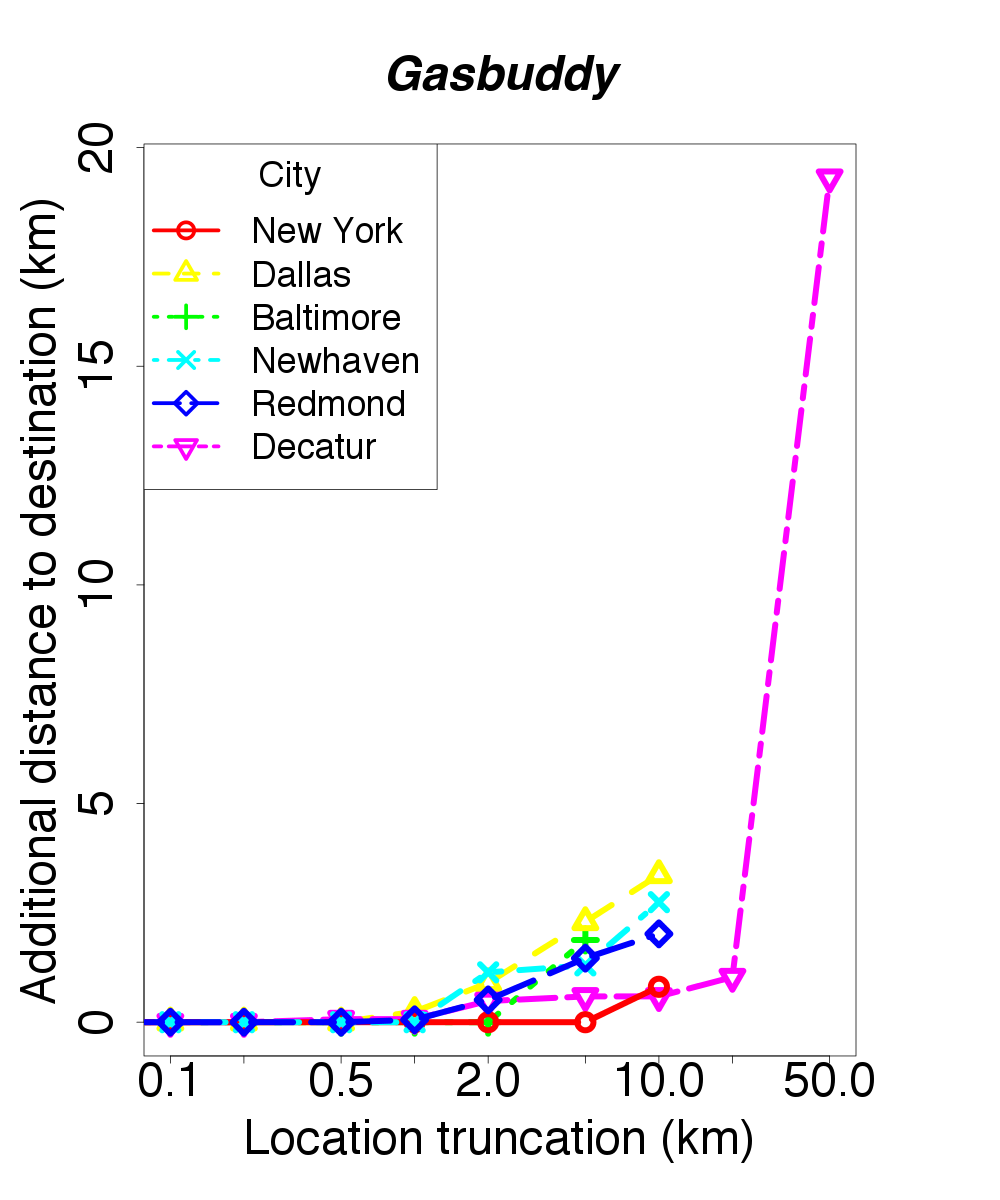
\includegraphics[width=\textwidth]
                      {location_privacy/data/gasbuddy/plots/medians_across_city_additional_distance}
    \end{minipage}
    
    % [width=.6\textwidth]
    \begin{minipage}{2in}
      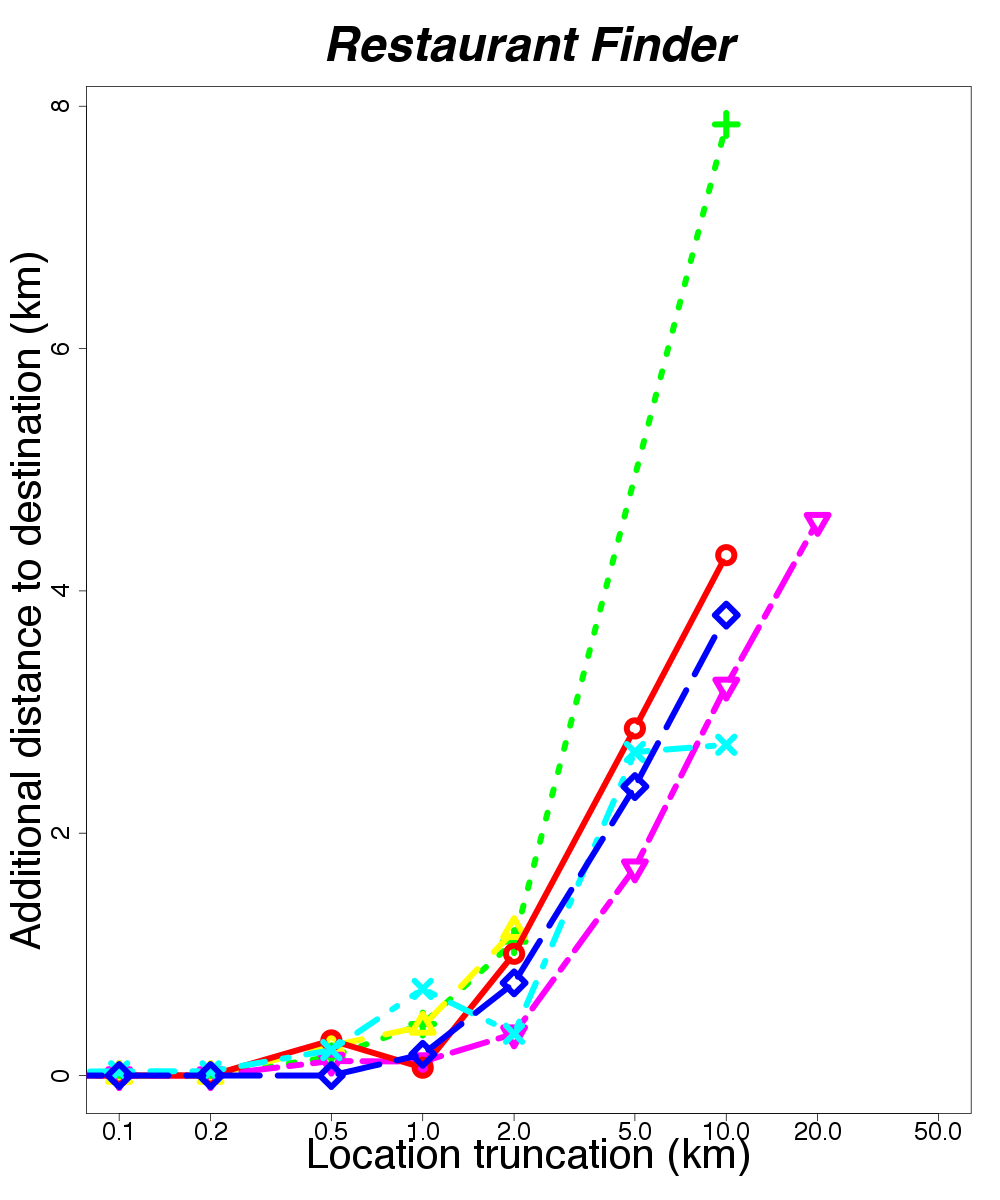
\includegraphics[width=\textwidth]
                      {location_privacy/data/restaurant_finder/plots/medians_across_city_additional_distance}
    \end{minipage}
    
    \begin{minipage}{2in}
      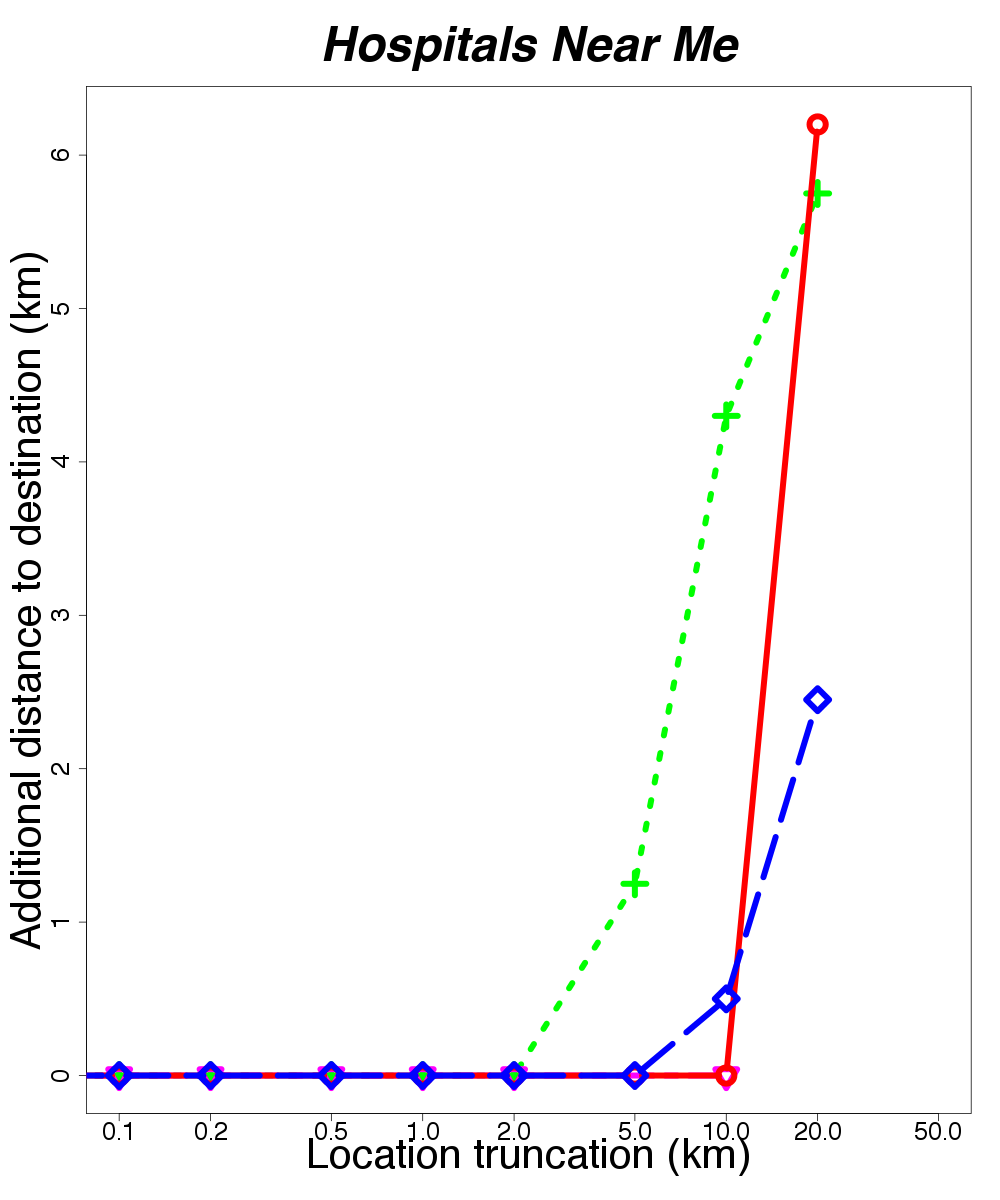
\includegraphics[width=\textwidth]
                      {location_privacy/data/hospitals/plots/medians_across_city_additional_distance}
    \end{minipage}
    
    \\
    \begin{minipage}{2in}
      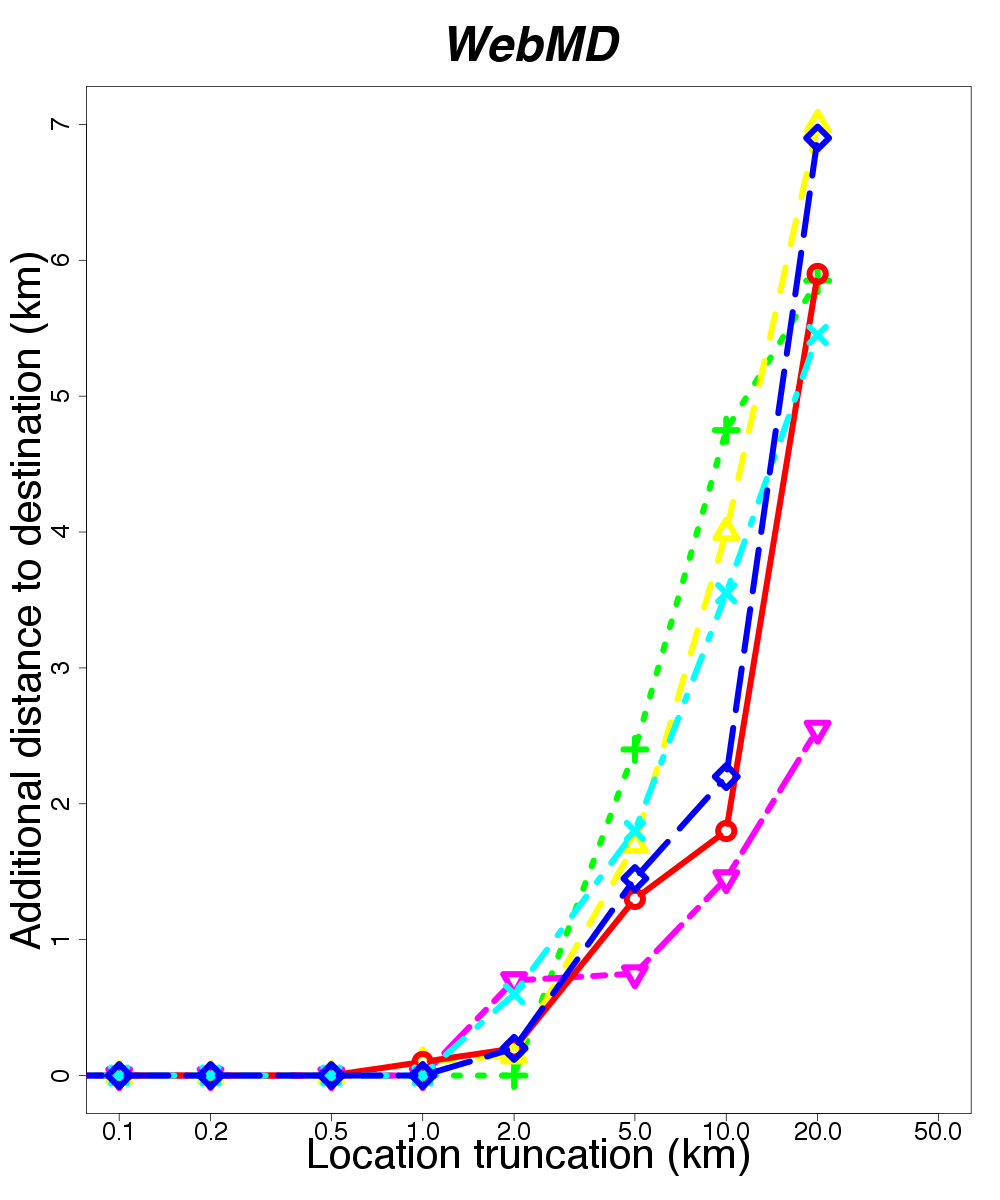
\includegraphics[width=\textwidth]
                      {location_privacy/data/webmd/plots/medians_across_city_additional_distance}
    \end{minipage}
    
    \begin{minipage}{2in}
      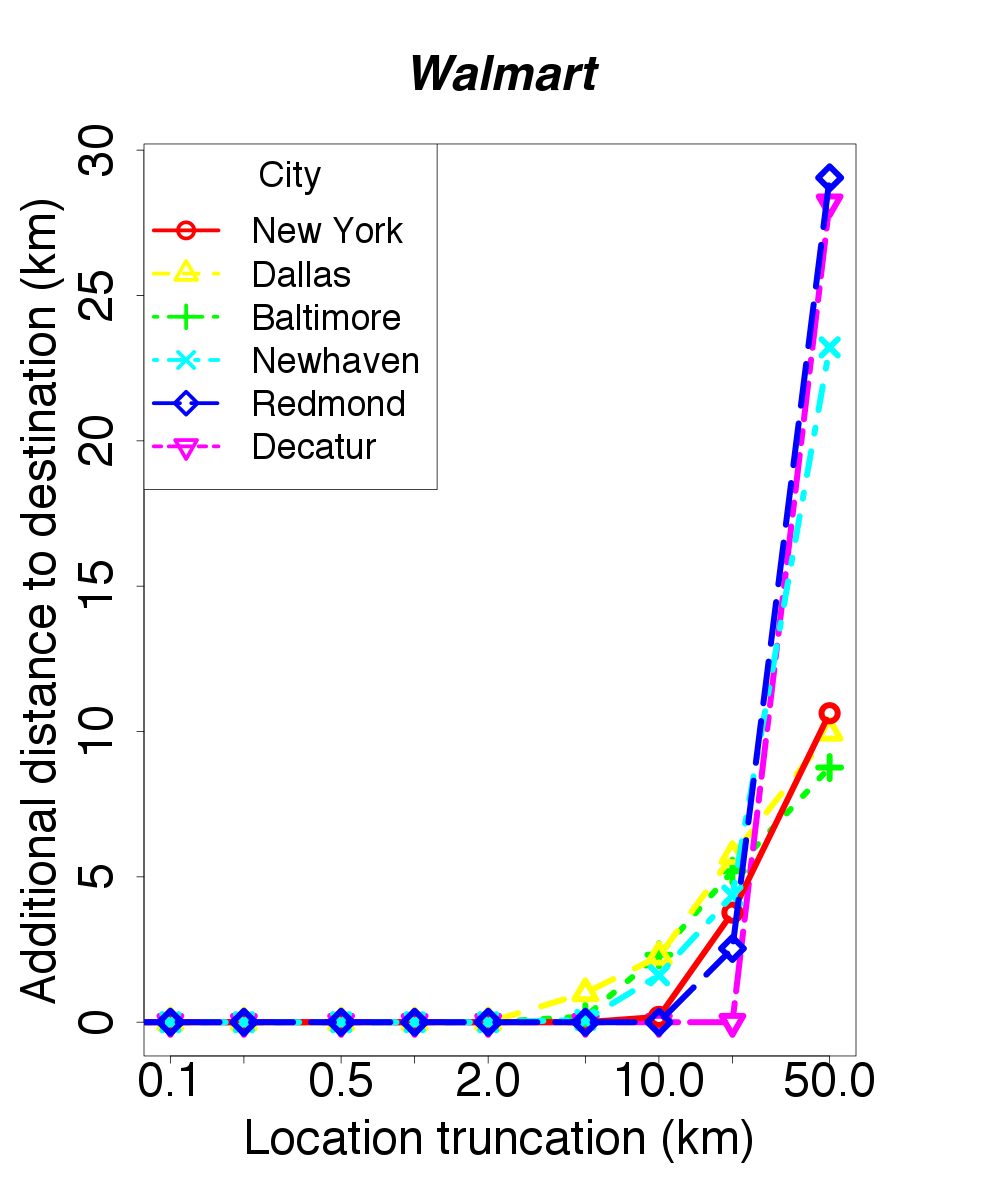
\includegraphics[width=\textwidth]
                      {location_privacy/data/walmart/plots/medians_across_city_additional_distance}
    \end{minipage}
    
    \begin{minipage}{2in}
      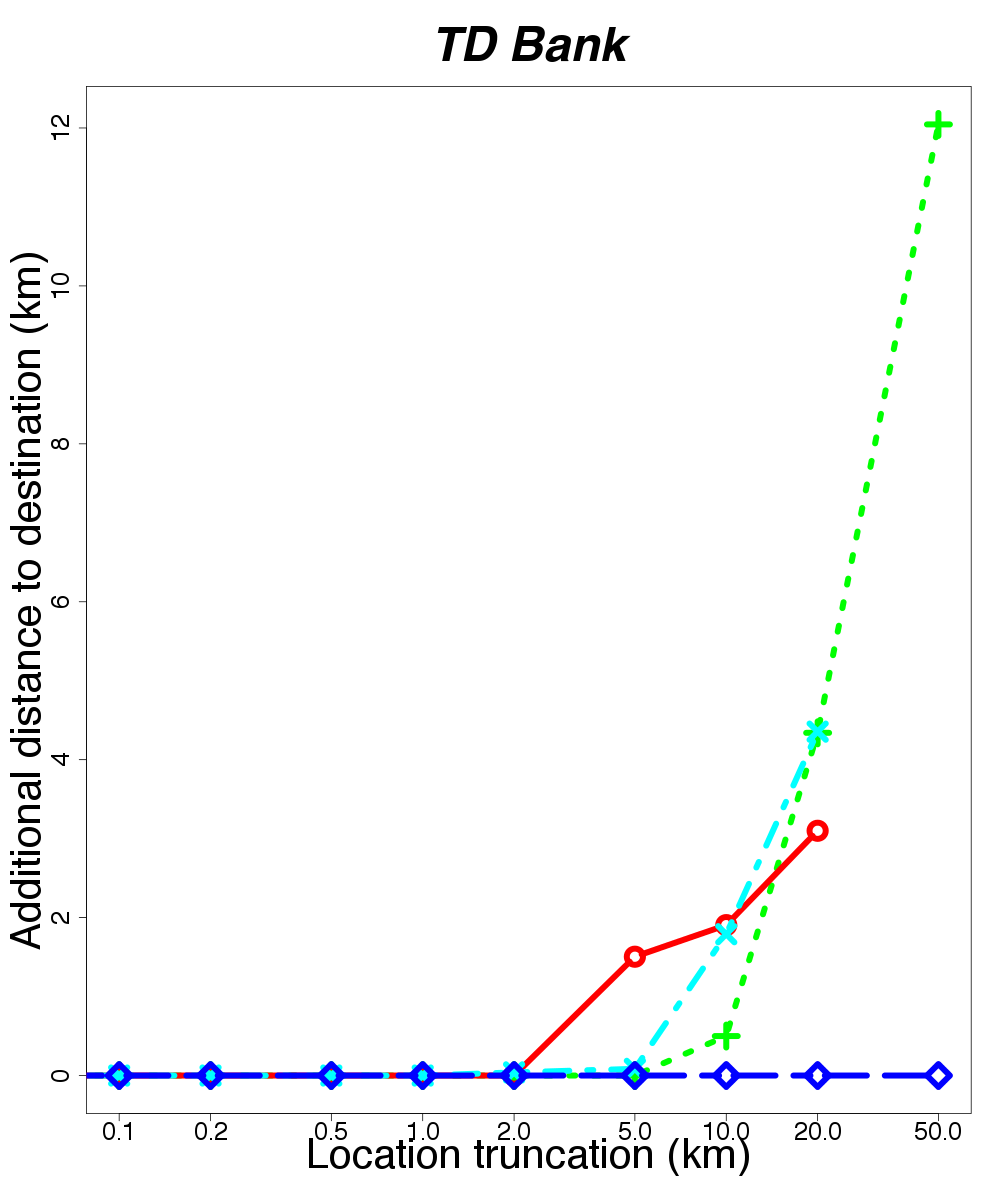
\includegraphics[width=\textwidth]
                      {location_privacy/data/tdbank/plots/medians_across_city_additional_distance}
    \end{minipage}
  \end{tabular}
  \caption{Graph of median additional distance versus
    truncation amount.  Higher additional distance implies lower
    utility.}
  \label{fig:add_distance}
  \end{subfigure}

  \bigskip{}

  \begin{subfigure}[t]{\textwidth}
 \small
 \centering
 \begin{tabular}{|l|rrrrrr|}
 \hline
 & New York & Dallas & Baltimore & New Haven & Redmond & Decatur \\
 \hline
 Gasbuddy & $\cdot$ & 5 & 5 & 2 & 5 & 20 \\
Restaurant Finder & 2 & 2 & 2 & 5 & 5 & 5 \\
Walmart & 20 & 5 & 10 & 10 & 20 & 50 \\
TD Bank & 5 & $\cdot$ & 20 & 10 & $\cdot$ & $\cdot$ \\
WebMD & 5 & 5 & 5 & 5 & 5 & 10 \\
Hospitals Near Me & 20 & $\cdot$ & 5 & $\cdot$ & 20 & $\cdot$ \\
\hline
\end{tabular}
\caption{Largest truncation amount (km) before median additional
  distance exceeds 1~km.}
 \label{fig:knee-points-additional-cutoff}

  \end{subfigure}

\caption{Additional distance results.}
  
\end{figure*}

\subsubsection{Set Intersection}

Figure~\ref{fig:set-intersection-metric} shows the results for the set
intersection size metric, with the $y$-axis the percentage of the set
intersection size compared to the original set size.
Figure~\ref{fig:knee-points-set-cutoff} shows the truncation amount
after which the set intersection percentage drops below 80\% of the
original value.  More precisely, let $I(s)$ be the median intersection
set size under truncation $s$, defined as $|L \cap L'|/|L|$ where $L$
is the list without truncation and $L'$ is the list with truncation
$s$. Then the chart lists the $s_i$ such that $I(s_i) \leq 0.8$ and
$I(s_{i+1}) > 0.8$, where $s_j$ is the sequence of location truncation amounts.

We observe that apps measuring less densely distributed locations can
be truncated more aggressively than those measuring more densely
distributed locations.
For example, we see that Gasbuddy and Restaurant Finder,
which both measure densely distributed objects,
can sustain some truncation, but their utility drops off much faster than the
other apps such as Hospitals Near Me. In the table, we see this again
in that Gasbuddy and Restaurant Finder drop
below a set intersection size of 80\% at a lower truncation amount compared to Hospitals Near Me.

One slightly surprising trend in the table is that for Restaurant
Finder, location can be truncated more in New York than in other
location, whereas we would expect the opposite due to its
high density of restaurants. Looking into the results in detail, we
discovered this occurred because of the large radius (20~km) we chose
for New York: Restaurants are
typically clustered in the city center and we chose
locations randomly within the radius, so a large radius reduced restaurant
density.

\subsubsection{Additional Distance}

Figure~\ref{fig:add_distance} shows the results for the additional
distance metric applied to our subject apps.
Figure~\ref{fig:knee-points-additional-cutoff} shows, for each city
and each app, the last truncation amount before median additional
distance degrades beyond 1~km. In other words, if we let
$\Delta(s)$ be the
median additional distance under truncation $s$, the chart lists
the $s_i$ such that $\Delta(s_i) \leq 1~km$ and $\Delta(s_{i+1}) >
1~km$.

Note that the additional distance is undefined if a location
truncation produces a new closest location that was not present in the
original output list, as in this case we cannot compute how far the
new closest location is from the current location. In the charts,
undefined additional distances are omitted, as thus some lines end
before reaching the maximum truncation. This also limits the number of
points on which we can compute the cutoff.  For example, the Gasbuddy
app never causes the user to go more than 1 km out of the way in New York, 
so it is listed as ``$\cdot$'' in Figure~\ref{fig:knee-points-additional-cutoff}.

From these plots, we see that under the additional distance
metric, there is typically no change in app utility up to 1 or 2~km
truncation. Notice that this is
quite different behavior than under the edit distance metric,
where the edit distance is nonzero even with small amounts of 
location truncation.

In most cases, the lack of change in additional distance is
meaningful, but in a few cases it only reveals the low density of
located objects. In particular, in Redmond, the TD Bank app can
sustain location truncation up to 50~km without any change, but
this occurs because the first result on the list is over 100 km~away. This
also happens in the Hospitals Near Me app, as there are relatively few
hospitals in any area.

Looking at Figure~\ref{fig:knee-points-additional-cutoff}, we see that
if a user is willing to go 1~km out of their way, then in most
locations apps can sustain truncation amounts of 5~km or
more. However, as with edit distance the effect is highly dependent on
object density, e.g., Gasbuddy and Restaurant Finder are limited to 5~km
truncation (except in Decatur, which has fewer gas
stations), whereas other apps can be truncated to higher levels.

\subsubsection{Discussion}

Each of the three metrics applies in a different situations: edit
distance for when an exact order is desired, set intersection for when
a user wants to find any number of locations close by, and additional
distance for when a user wants to find a nearest location to visit.
The general trend for all three are similar: the metrics are much
more forgiving in less dense areas, which makes intuitive sense. In
terms of absolute values of truncation that can be sustained, we see
that edit distance is the least permissive, as very small changes have
large effects. (We did not include a table like
Figure~\ref{fig:knee-points-additional-cutoff}
or~\ref{fig:knee-points-set-cutoff} for edit distance because we have
no intuition of what a reasonable cutoff would be.) The next most
restrictive metric is set intersection size, and the most permissive
metric is additional distance.

\section{Related Work}

Several other researchers have proposed mechanisms to refine or reduce
permissions in Android. MockDroid allows users to replace an
app's view of certain private data with fake
information~\cite{mockdroid}. Apex is similar, and also lets 
the user enforce simple constraints such as the
number of times per day a resource may be accessed~\cite{apex}. TISSA
gives users detailed control over an app's access to selected private data
(phone identity, location, contacts, and the call log), letting the
user decide whether the app can see the true data, empty data,
anonymized data, or mock data~\cite{zhou2011taming}. AppFence
similarly lets users provide mock data to apps requesting private
information, and can also ensure private data that is released to apps
does not leave the device~\cite{Hornyack:2011}.  A
limitation of all of these approaches is that they require
modifications to the Android platform, and hence to be used in
practice must either be
adopted by Google or device providers, or must be run on rooted
phones. In contrast, \rewriter and \lib run on stock, unmodified
Android systems available today.

Researchers have also developed other ways to enhance Android's
overall security framework. Kirin employs a set of user-defined
security rules to flag potential malware at install
time~\cite{enck2009lightweight}. Saint enriches permissions on Android
to support a variety of installation constraints, e.g., a permission
can include a whitelist of apps that may request
it~\cite{ongtang2009semantically}. These approaches are complementary
to our system, as they take the platform permissions as is and do not
refine them.

There have been several studies of Android's permissions, sensitive
APIs, and the use of permissions across apps.  Barrera et
al.~\cite{barrera2010methodology} analyze the way permissions are used
in Android apps, and observe that only a small number of Android
permissions are widely used but that some of these, in particular
Internet permissions, are overly broad (as we have also found). Vidas
et al.~\cite{vidas:w2sp11} describe a tool that, using
documentation-derived information, can statically analyze an app's
source code to find a minimum set of permissions it
needs. Stowaway~\cite{Felt:2011} performs a static analysis on the
Android API itself to discover which APIs require what permissions,
something they found is not always well documented. (We used
Stowaway's data set in several cases to help determine what adapters
we needed to implement in \lib.)

Finally, several tools have been developed that look for security
issues in Android apps. TaintDroid tracks the flow of sensitive
information~\cite{taintdroid}. Ded~\cite{ded}, a Dalvik-to-Java
decompiler, has been used to discover previously undisclosed device
identifier leaks. ComDroid~\cite{chin11:mobisys} finds vulnerabilities
related to Intent handling. Felt et al.~\cite{felt2011permission}
study the problem of permission redelegation, in which an app is
tricked into providing sensitive capabilities to another app.
Woodpecker~\cite{grace:ndss12} uses dataflow analysis to find
capability leaks on Android phones. All of these tools focus on
improper use of the current set of Android's permissions. \rewriter
and \lib take a complimentary approach, replacing existing permissions
with finer-grained ones to reduce or eliminate consequences of
security issues.

\paragraph*{Related Work for Location Privacy}

There is a large body of work on increasing location
privacy, though we are aware of no other work that directly measures
the resulting utility of mobile Android apps.

The Cach\'{e} system \cite{Amini:2010} caches and prefetches
content from a server, obfuscating the user's location at the cost of
potentially stale content and higher bandwidth.  Additionally,
application writers must specify rules for caching up front.  The
system caches data for a set of regions, quantizing the user's location 
as in our approach.  
The authors note that app utility will be impacted by their technique, 
but they do not measure it explicitly.

Hornyack et al. \cite{Hornyack:2011} study apps that use sensitive
information (such as location), and present AppFence, a system that
can fuzz inputs to apps. While the AppFence authors note the effects of
fuzzing app inputs on usability, they do not study it systematically
using any particular metric.

Shokri et al. \cite{Shokri:2011} present a systematic approach to
quantifying Location Privacy Preserving Mechanisms (LPPMs).  They also
describe an meter on the user's devise that
continuously informs the user of their privacy.  In our work, we implemented a simple
truncation-based LPPM (corresponding to a technique they call
\emph{precision reduction}), and use this to study
utility as a function of the degree of truncation. As future work, we
may consider evaluating the utility of other policies from their
system.

In follow up work, Shokri et al. \cite{Shokri:2012} present an
optimal strategy to prevent localization attacks.
%, based on bounding
%the probability that an attacker can learn the
%precise location of a user at a given time.  
Their analysis formulates location privacy as a Bayesian Stackelberg 
game, where a user chooses a location cloaking strategy without 
knowing their potential adversary.
While their analysis considers service quality, they use metrics that do 
not clearly map to utility, such as Euclidean distance from the 
true location (rather than the actual effect of the change on the service).

Our study focuses on privacy for a single user at a stationary point.
Allowing the app to collect traces of data reveals much more
information \cite{Gruteser:2005}, \cite{Golle:2009}.  Much of the
existing work on location privacy \cite{Beresford:2004}, \cite{Bettini:2005},
\cite{Hoh:2005}, \cite{Gruteser:2003} focuses on $k$-anonymity: if a
user is making a query to a location based service, they can only be
identified to be within a set of $k$ potential users.  
One popular
technique is to use mix zones \cite{Beresford:2004}: once a user enters 
a designated area their location information becomes ``mixed'' with 
others in that same area.  This technique requires a trusted middleware 
layer (to properly mix location data) and requires these mix zones 
to be defined.  In contrast, location truncation can be done locally
on a mobile device.

None of these previous approaches study the impact of location privacy
on app utility.  The work that comes closest is by Shokri et
al. \cite{Shokri:2012}, but while that framework considers utility as
an element of their models, it is not directly measured on apps.  Our
work is complementary: we focus not on optimal obfuscation techniques,
but rather we fix an obfuscation strategy and study how utility
changes under that technique.  As future work, we intend to couple our 
empirical utility functions with the theoretical models presented by
Shokri et al.
Doing so would allow us to determine bounds for $k$ and allow us to study 
how the optimal strategies presented by Shokri et al.
are affected.

\section{Conclusion}

We presented an empirical study of how location truncation affects
mobile app utility. We began by examining how Android apps use
location. Across the apps we looked at, we found that the second most
common pattern is using the current location to list various sorts of
nearby objects. The most common pattern, location-targeted ads, is not
amenable to evaluating utility. We then used Dr.~Android and Mr.~Hide
to implement \fuzzer{}, a tool that
modifies existing apps' bytecode to use truncated location
information. We designed an experiment in which we measured the effect
of a range of location truncations (from 0~km to 50~km) on 60
points randomly chosen from various locales (from population 6,000
Decatur, TX to population 8.2 million New York, NY). We identified three
metrics that approximate app utility: edit distance, set intersection
size, and additional distance. We found that, under these metrics, the
factor that most determines the utility--truncation tradeoff is
the density of objects being returned by the app, and that in many
cases, location can be truncated significantly without losing much
utility. To our knowledge, our work provides the first end-to-end
evaluation of how location truncation affects Android app utility.
As subject of future work, we plan to apply CloakDroid to a larger 
number of apps and test the metrics using user studies.
